% !TeX root = ../libro.tex
% !TeX encoding = utf8
%
%*******************************************************
% Series Temporales
%*******************************************************

\chapter{Series Temporales}\label{ch:st}

Presentamos y explicamos la teoría sobre las \textbf{series temporales}, los objetos de estudio que se presentarán en nuestros problemas y que se usarán en los modelos realizados.

Usaremos como base para desarrollar esta parte la literatura para series temporales y procesos estocásticos, concretamente de \cite{cox1977theory}, \cite{chatfield2019analysis}, \cite{brockwell2002introduction}, \cite{hyndman2018forecasting}, \cite{box2011time} y \cite{grandell1998time}.

\section{Definición y características}

Para ver qué es y poder estudiar una serie temporal necesitamos tener una base de la teoría de \textbf{procesos estocásticos}. Esta teoría se encarga de estudiar sistemas que evolucionan en el \textbf{tiempo} en función de \textbf{leyes probabilísticas}.

\subsection{Elementos básicos}

Para explicar estos conceptos vamos a hacer un breve recordatorio de los elementos fundamentales que juegan un papel en la teoría de la probabilidad, que se basa en el estudio de ciertas \textbf{funciones} reales que parten de un espacio donde hay una \textbf{medida de probabilidad}.

La idea del espacio que hemos mencionado es muy simple: queremos asignar a \textbf{subconjuntos} (sucesos) de cierto \textbf{espacio} una cantidad numérica que representa la \textbf{probabilidad} de que ocurran. Por tanto necesitaremos un espacio $\Omega$, una $\sigma$-álgebra $\mathcal{A}$ sobre $\Omega$ (\autoref{def:sigma-algebra}) y una función de probabilidad $P$ en $\Omega$ (\autoref{def:probabilidad}).

\begin{definicion}[$\sigma$-álgebra]
  Sea un conjunto $\Omega$, una $\sigma$-álgebra sobre $\Omega$ es una familia $\mathcal{A}$ de subconjuntos de $\Omega$ que incluye el espacio entero y es cerrada bajo complementos y uniones numerables; es decir, que cumple lo siguiente:
  \begin{enumerate}
    \item $\Omega \in \mathcal{A}$.
    \item $\forall A \in \mathcal{A} \implies \overline{A} \in \mathcal{A}$.
    \item $\forall \{A_n\}_{n \in \N} \subseteq \mathcal{A} \implies \bigcup \limits^\infty_{n = 1} A_n \in \mathcal{A}$
  \end{enumerate}
  \label{def:sigma-algebra}
\end{definicion}

\begin{definicion}[Función de probabilidad]
  Sea un espacio $\Omega$, y $\mathcal{A}$ una $\sigma$-álgebra sobre $\Omega$, una función de probabilidad $P : \mathcal{A} \to R$ es una función que cumple lo siguiente:

  \begin{itemize}
    \item (No negativa): $\forall A \in \mathcal{A}, \, P(A) \geq 0$
    \item (Normalización): $P(\Omega) = 1$
    \item ($\sigma$-aditividad): $\forall \{A\}_{n \in \N} \subseteq \mathcal{A}$ disjuntos 2 a 2 $\implies P \left(\bigcup \limits^\infty_{n = 1} A_n \right) = \sum \limits^\infty_{n = 1} P(A_n)$
  \end{itemize}
  \label{def:probabilidad}
\end{definicion}

Juntando estos tres elementos obtenemos nuestro \textbf{espacio probabilístico} (\autoref{def:espacio-probabilistico}).

\begin{definicion}[Espacio probabilístico]
  Sea $\Omega$ un conjunto, $\mathcal{A}$ una $\sigma$-álgebra sobre $\Omega$ y $P$ una probabilidad en $\Omega$, entonces definimos el espacio de probabilidad como la terna $(\Omega, \mathcal{A}, P)$.
  \label{def:espacio-probabilistico}
\end{definicion}

Como la probabilidad $P$ es realmente una medida normalizada, podemos aplicar aspectos de la teoría de la medida en un espacio probabilístico. En concreto consideraremos funciones medibles, que son aplicaciones medibles (\autoref{def:aplicacion-medible}) donde el espacio de llegada es un espacio \textbf{Borel} ($\sigma$-álgebra formada con las semirrectas cerradas por la derecha $(-\infty, x]$).

\begin{definicion}[Aplicación medible]
  Sean dos espacios medibles $(\Omega_1, \mathcal{A}_1)$, $(\Omega_2, \mathcal{A}_2)$, una aplicación $f : \Omega_1 \to \Omega_2$ se dice medible, si y solamente si:

  $$\forall A \in \mathcal{A}_2, \, f^{-1}(A) = \{\omega \in \Omega_1 : f(\omega) \in A\} \in \mathcal{A}_1$$
  \label{def:aplicacion-medible}
\end{definicion}

Definimos así las funciones que forman la base de esta teoría: las \textbf{variables aleatorias} (\autoref{def:var-aleatoria}). Hemos tomado el espacio Borel usual como $(\R, \mathcal{B})$ aunque si tenemos un subconjunto $E \subseteq \R$ se puede considerar el espacio Borel $(E, \mathcal{B}_E)$ donde $\mathcal{B}_E$ es la $\sigma$-álgebra Borel restringida a $E$.

\begin{definicion}[Variable aleatoria]
  Sea un espacio de probabilidad $(\Omega, \mathcal{A}, P)$, una variable aleatoria es una función medible de un espacio de probabilidad en un espacio Borel $X: (\Omega, \mathcal{A}, P) \to (\R, \mathcal{B})$.
  \label{def:var-aleatoria}
\end{definicion}

Una variable aleatoria $X$ induce una probabilidad en el espacio de llegada Borel que denominamos como \textbf{función de probabilidad} (\autoref{def:distribucion-probabilidad}).

\begin{definicion}[Distribución de probabilidad]
  Sea un espacio probabilístico $(\Omega, \mathcal{A}, P)$ y una variable aleatoria $X: (\Omega, \mathcal{A}, P) \to (\R, \mathcal{B})$, llamamos distribución de probabilidad de una variable aleatoria a una función de probabilidad definida en el espacio Borel, dada por:

  $$\begin{aligned} P_X : \mathcal{B} & \to \R \\
      B & \mapsto P_X(B) = P(X^{-1}(B)) = P[X \in B]
    \end{aligned}.$$
  \label{def:distribucion-probabilidad}
\end{definicion}

Si recordamos, la $\sigma$-álgebra Borel $\mathcal{B}$ estaba generada por las semirrectas abiertas por la derecha ($(-\infty, x]$), por lo que podemos definir la distribución como una función de variable real: \textbf{ffunción de distribución} (\autoref{def:funcion-distribucion}).

\begin{definicion}[Función de distribución]
  Sea un espacio probabilístico $(\Omega, \mathcal{A}, P)$ y una variable aleatoria $X: (\Omega, \mathcal{A}, P) \to (\R, \mathcal{B})$, Llamamos función de distribución a la función definida de la siguiente forma:

  $$\begin{aligned} F_X : \R & \to \R \\
      x & \mapsto F_X(x) = P_X((-\infty, x]) = P[X \leq x]
    \end{aligned}.$$
\label{def:funcion-distribucion}
\end{definicion}

Cabe añadir que todo lo que hemos visto de teoría es fácilmente extensible al caso multidimensional (cuando el espacio Borel es multidimensional $R^n$) ya que se considera $X = (X_1, \ldots, X_n)$ como un \textbf{vector aleatorio} donde $X_i$ es una variable aleatoria $i = 1, \ldots, n$.

\subsection{Procesos estocásticos}

Ya podemos definir qué es un \textbf{proceso estocástico}, que no es más que una sucesión de variables aleatorias ordenadas por el tiempo (\autoref{def:proceso-estocastico}).

\begin{definicion}[Proceso estocástico]
  Sea un espacio de probabilidad $(\Omega, \mathcal{A}, P)$, un conjunto ordenado arbitrario $T$, un espacio Borel $(E, \mathcal{B}_E)$ y las variables aleatorias $X_t : (\Omega, \mathcal{A}, P) \to (\R, \mathcal{B}), \, \forall t \in T$. Un proceso estocástico es una familia de variables aleatorias $\{X_t\}_{t \in T}$ ordenadas por $T$.
  \label{def:proceso-estocastico}
\end{definicion}

Notamos $T$ como el \textbf{espacio paramétrico} y es a lo que nos referimos como el tiempo. Según quién sea $T$ podemos decir que el proceso es en \textbf{tiempo discreto} ($T = \N \cup \{0\}$) o en \textbf{tiempo continuo} ($T = [0, + \infty)$). Además, el espacio Borel de llegada se denomina como \textbf{espacio de estados} y nos permite clasificar el proceso como \textbf{discreto} (si $E$ es discreto) o \textbf{continuo} (si $E$ es no numerable).

Listamos unos cuantos ejemplos ilustrativos de procesos estocásticos:

\begin{itemize}
  \item Discreto:
    \begin{itemize}
      \item En tiempo discreto: lanzar un dado numerado del 1 al 6 y anotar el resultado. $X_n$ es el resultado del lanzamiento $n$-ésimo, $E = \{1, 2, 3, 4, 5, 6\}$ y $T = \N$.
      \item En tiempo continuo: contar el número de personas en una tienda en un instante. $X_t$ es el número de personas en el instante $t$, $E = \N$ y $T = \R^+_0$.
    \end{itemize}
  \item Continuo:
    \begin{itemize}
      \item En tiempo discreto: medir la cantidad de agua promedio de lluvia en una ciudad cada día. $X_n$ es la cantidad de agua promedio de lluvia en el dia $n$, $E = \R^+_0$ y $T = \N$.
      \item En tiempo continuo: medir la posición de un objeto móvil en un instante. $X_t$ es la posición del objeto en el instante $t$, $E = \R$, $T = \R^+_0$.
    \end{itemize}
\end{itemize}

Así una \textbf{serie temporal} no será nada más que una \textbf{realización}, una muestra, de un proceso estocástico (\autoref{def:serie-temporal}). Un ejemplo lo encontramos en \autoref{fig:ej-ts} \cite{brockwell2002introduction}.

\begin{figure}[htpb]
  \centering
  %\hspace*{-2.5cm}
  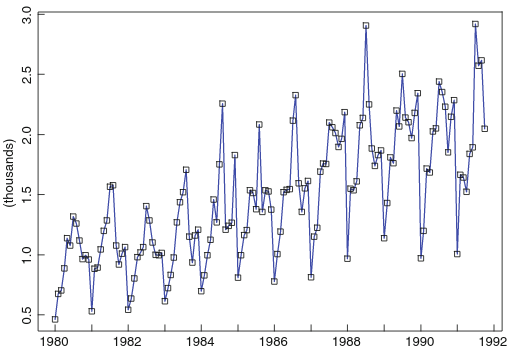
\includegraphics[width=.6\textwidth]{ej-ts}
  \caption{Ejemplo de serie temporal continuo en tiempo discreto. Ventas de vino tinto en Australia 1980-1991.}
  \label{fig:ej-ts}
\end{figure}

\begin{definicion}[Serie temporal]
  Sea un proceso estocástico $\{X_t\}_{t \in T}$, con $X_t : (\Omega, \mathcal{A}, P) \to (E, \mathcal{B}_E), \, \forall t \in T$. Una serie temporal es una realización del proceso estocástico $\{x_t : x_t \in E, t \in T \}$
  \label{def:serie-temporal}
\end{definicion}

Tenemos en cuenta que al hacer una realización obtendremos siempre una cantidad de puntos finitos, que no es excluyente con el hecho de que venga de un proceso en tiempo continuo mientras se haga un muestreo correcto. Además, sea el proceso en tiempo discreto o continuo, generalmente se considera que los tiempos en los que se obtiene la muestra están separados uniformemente.

\subsection{Momentos}

El estudio de los procesos y de las series está profundamente ligado a la predicción de valores: si conseguimos modelar y captar la estructura del proceso podremos predecir valores para tiempos en el futuro. Sin embargo, en general necesitaremos conocer las distribuciones $n$-dimensionales del proceso dadas por la distribución de probabilidad conjunta \eqref{eq:distri-multidim}

\begin{equation}
  P[X_{t_1} \leq x_{t_1}, \ldots, X_{t_n} \leq x_{t_n}], \; \forall \{t_i\}^n_{i = 1} \subseteq T, \; \forall n \in \N.
  \label{eq:distri-multidim}
\end{equation}

Esto en la práctica es muy complicado y poco fáctible de obtener, ya que usualmente solo se tiene una única serie temporal del proceso. Una manera más fácil y útil de describir un proceso es mediante los \textbf{momentos}, en particular los momentos de primer y segundo orden que son las funciones \textbf{media} (\autoref{def:func-media}) y \textbf{autocovarianza} (\autoref{def:func-autocovarianza}) respectivamente.

\begin{definicion}[Función media]
  Sea un proceso estocástico $\{X_t\}_{t \in T}$ que cumple que $E[X_t] < +\infty, \, \forall t \in T$. La función media del proceso se define como:

  $$\begin{aligned} \mu : T & \to \R \\
    t & \mapsto \mu(t) = E[X_t]
  \end{aligned}.$$
  \label{def:func-media}
\end{definicion}

\begin{definicion}[Función autocovarianza]
  Sea un proceso estocástico $\{X_t\}_{t \in T}$ que cumple que $Var[X_t] < +\infty, \, \forall t \in T$. La función media del proceso se define como:

  $$\begin{aligned} \gamma : T \times T & \to \R \\
    (t_1, t_2) & \mapsto \gamma(t_1, t_2) = E\left[(X_{t_1} - \mu(t_1))(X_{t_2} - \mu(t_2))\right] = Cov(X_{t_1}, X_{t_2})
  \end{aligned}.$$
  \label{def:func-autocovarianza}
\end{definicion}

Podemos definir la función \textbf{varianza} como un caso especial de la función autocovarianza cuando $t_1 = t_2$, es decir $\sigma^2(t) = \gamma(t_1, t_1) = Var[X_t]$.

\subsection{Procesos estacionarios}

Una propiedad muy interesante y que puede ayudarnos al modelar los procesos, es cuando es \textbf{estacionario}. De manera informal, un proceso es estacionario si sus propiedades estadísticas (momentos) no cambian con el tiempo.

Veamos que significa formalmente que un proceso sea \textbf{estrictamente estacionario} (\autoref{def:estrictamente-estacionario}).

\begin{definicion}[Proceso estrictamente estacionario]
  Un proceso estocástico $\{X_t\}_{t \in T}$ se dice que es estrictamente estacionario si $\forall n \in N$, $\forall t_1 < \ldots < t_n \in T$, $\forall \tau \in T$ se cumple que:

    $$\left( X_{t_1}, \ldots, X_{t_n}\right) \sim \left( X_{(t_1 + \tau)}, \ldots, X_{(t_n + \tau)}\right).$$
  \label{def:estrictamente-estacionario}
\end{definicion}

Lo que nos dice esta propiedad es que la probabilidad conjunta no cambia si se desplaza, por lo que solo dependerá de la probabilidad conjunta para $t_1, \ldots, t_n$, $\forall n \in N$. De hecho si $n=1$ tendremos que los momentos, si existen, serán todos iguales \eqref{eq:estricto-momentos}

\begin{gather}
  \mu(t) = \mu, \\
  \sigma^2(t) = \sigma^2.
  \label{eq:estricto-momentos}
\end{gather}

Además, si $n = 2$ entonces la distribución conjunta de $X_{t_1}$ y $X_{t_2}$ dependerá solo de la diferencia temporal $(t_2 - t_1) = \tau$ denominada como \textbf{desfase} (\emph{lag}). Por tanto la función autocovarianza puede ser reescrita en función únicamente del desfase, denominándose como \textbf{coeficiente de autocovarianza} con desfase $\tau$ \eqref{eq:estricto-autocovarianza}

\begin{equation}
  \gamma(t_1, t_2) = Cov(X_{t_1}, X_{t_2}) = Cov(X_{0}, X_{(t_2 - t_1)}) = \gamma(0, \tau) = \gamma(\tau).
  \label{eq:estricto-autocovarianza}
\end{equation}

Como las dimensiones del coeficiente de autocovarianza depende de las unidades de medida de $X_t$, por motivos de interpretabilidad se suele estandarizar obteniendo así la función de \textbf{autocorrelación} (ACF) que mide la correlación entre $X_t$ y $X_{t + \tau}$ \eqref{eq:autocorrelacion}

\begin{equation}
  \rho(\tau) = \dfrac{\gamma(\tau)}{\gamma(0)}.
  \label{eq:autocorrelacion}
\end{equation}

Aunque pareciera que no existen muchos procesos que mantengan la misma distribución en todo el tiempo, si existen muchos procesos con una distribución \textbf{de equilibrio}. Estos procesos cumplen que la distribución de probabilidad de $X_t$ tiende a una distribución limite (de equilibrio) cuando $t \to \infty$ y no dependen de las condiciones iniciales. Por tanto si las condiciones iniciales se fijan para ser iguales que la distribución de equilibrio, el proceso es fuertemente estacionario.

Sin embargo, podemos relajar las condiciones de la propiedad para hacerlas más prácticas en casos reales, únicamente con condiciones a los momentos de primer y segundo orden. Definimos los procesos \textbf{débilmente estacionarios} o \textbf{estacionarios de segundo orden} como \autoref{def:debilmente-estacionario}.

\begin{definicion}[Proceso estacionario de segundo orden]
  Sea un proceso estocástico $\{X_t\}_{t \in T}$, se dice que el proceso es débilmente estacionario o estacionario de segundo orden si se cumple lo siguiente:

  \begin{enumerate}
    \item $\mu(t) = \mu, \, \forall t \in T$.
    \item $\gamma(t_1, t_2) = \gamma  (t_1 + \tau, t_2 + \tau), \, \forall t_1, t_2, \tau \in T$
  \end{enumerate}

  La condición 2, como ya vimos, implica que $\gamma(t_1, t_2) = \gamma(\tau)$.
  \label{def:debilmente-estacionario}
\end{definicion}

Obviamente que un proceso sea fuertemente estacionario implica que sea débilmente estacionario pero no al revés. De hecho la doble implicación se da si el proceso tiene una distribución conjunta normal multivariante, ya que en ese caso queda determinada por los momentos de primer y segundo orden.

El \textbf{ruido independiente idénticamente distribuido} (ruido iid.) es el ejemplo básico de proceso estrictamente estacionario (\autoref{def:ruido-iid}).

\begin{definicion}[Ruido iid]
  Un proceso $\{X_t\}_{t \in T}$ estocástico se dice que es ruido independiente idénticamente distribuido con media $\mu$ y varianza $\sigma^2$, denotado por $\{X_t\} \sim IID(\mu, \sigma^2)$, si todas las variables aleatorias $X_t$ son independientes e idénticamente distribuidas con $E[X_t] = \mu, Var[X_t] = \sigma^2, \, \forall t \in T$.
\label{def:ruido-iid}
\end{definicion}

Debido a la independencia de las variables tendremos que la función media del proceso será $\mu$, y la función autocovarianza será \eqref{eq:autocov-ruido}

\begin{equation}
  \gamma(\tau) =
  \begin{cases}
    \sigma^2, & \tau = 0 \\
    0, & \tau \neq 0
  \end{cases},
  \label{eq:autocov-ruido}
\end{equation}

que no depende del tiempo $t$ y junto a la independencia de las variables nos dice que el proceso es estrictamente estacionario.

Uno puede relajar la condición de independencia e distribución idéntica para obtener un tipo de proceso estacionario de segundo orden, el llamado \textbf{ruido blanco} (\autoref{def:ruido-blanco}).

\begin{definicion}[Ruido blanco]
  Un proceso $\{X_t\}_{t \in T}$ estocástico se dice que es ruido blanco (\emph{white noise}) con media $\mu$ y varianza $\sigma^2$, denotado por $\{X_t\} \sim WN(\mu, \sigma^2)$, si todas las variables aleatorias $X_t$ son incorreladas con $E[X_t] = \mu, Var[X_t] = \sigma^2, \, \forall t \in T$.
\label{def:ruido-blanco}
\end{definicion}

En este caso el ruido blanco obtiene la misma función media y autocovarianza que el ruido iid. \eqref{eq:autocov-ruido} haciendo que el proceso sea estacionario de segundo orden. Así, cualquier proceso $IID(\mu, \sigma^2)$ es $WN(\mu, \sigma^2)$ pero no al revés.

Para ambos procesos podemos calcular la función de autocorrelación \eqref{eq:ruido-autocorrelacion}

\begin{equation}
  \rho(\tau) =
  \begin{cases}
    1, & \tau = 0 \\
    0, & \tau \neq 0
  \end{cases}.
  \label{eq:ruido-autocorrelacion}
\end{equation}

Mostramos un ejemplo de un proceso $\{X_n\}_{n = 1}^{500} \sim IID(0, 1)$ generado con $X_n \sim N(0, 1), \, n = 1, \ldots, 500$ junto con su correlograma (el valor de la función de autocorrelación en función del desfase) (\autoref{fig:ruido-ej}, \cite{chatfield2019analysis}).

\begin{figure}[htpb]
  \centering
  %\hspace*{-2.5cm}
  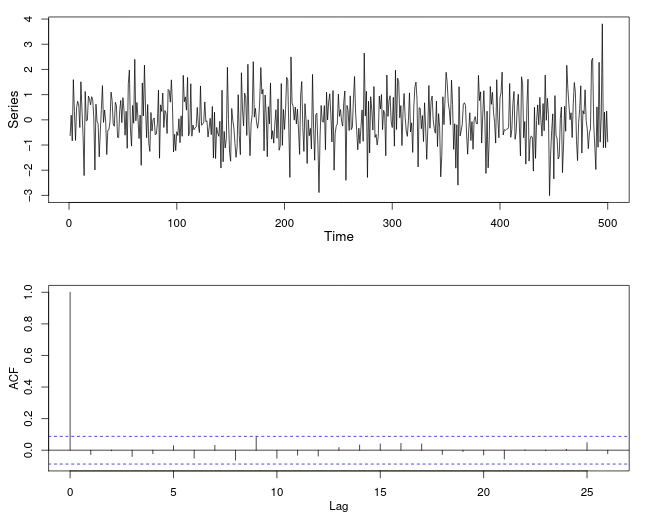
\includegraphics[width=.8\textwidth]{ruido-iid}
  \caption{Proceso $IID(0, 1)$ con su correlograma.}
  \label{fig:ruido-ej}
\end{figure}

Un proceso muy simple que no es estacionario es el \textbf{camino aleatorio} (\autoref{def:random-walk}).

\begin{definicion}[Camino aleatorio]
  Se dice que un proceso $\{X_t\}_{t \in T}$ es un camino aleatorio si

  $$X_t = X_{t - 1} + Z_t, \, \forall t \in T,$$

  donde $\{Z_t\}_{t \in T} \sim IID(\mu , \sigma^2)$. Generalmente cuando $t = 1$ se toma $X_1 = Z_1$, haciendo que el proceso sea como:

  $$X_t = \sum \limits^t_{i = 1} Z_i, \, \forall t \in T.$$
  \label{def:random-walk}
\end{definicion}

Para un camino aleatorio se tiene debido a la independencia de $Z_t$ que $E[X_t] = t \mu$ y $Var[X_t] = t \sigma^2$. Como dependen de $t$ el proceso no es estacionario.

Podemos generar caminos aleatorios fácilmente mediante un proceso $IDD(\mu, \sigma^2)$ (\autoref{fig:ej-random-walk}, \cite{chatfield2019analysis}).

\begin{figure}[htpb]
  \centering
  %\hspace*{-2.5cm}
  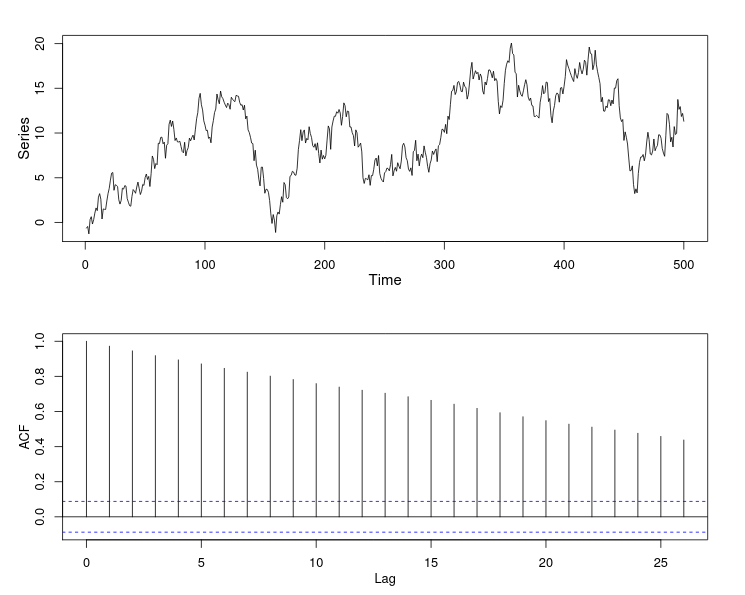
\includegraphics[width=.8\textwidth]{random-walk-ej}
  \caption{Ejemplo de camino aleatorio generado con ruido, junto con su correlograma.}
  \label{fig:ej-random-walk}
\end{figure}

\subsection{Propiedades de la funciones de autocovarianza y autocorrelación}

Finalmente veremos unas pocas propiedades interesantes sobre las funciones de autocovarianza $\gamma$ y autocorrelación $\rho$ de un proceso estacionario. Primero veamos las propiedades de la autocovarianza (\autoref{prop:propiedades-gamma}).

\begin{proposicion}[Propiedades de $\gamma$]
  Sea un proceso estacionario de segundo orden $\{X_t\}_{t \in T}$ con función de autocovarianza definida como

  $$\gamma(\tau) = Cov(X_{t + \tau}, X_t), \; \forall \tau \in T,$$

  entonces se cumplen las siguientes afirmaciones

  \begin{enumerate}
    \item $\gamma(0) = \sigma^2 \geq 0$.
    \item $|\gamma(\tau)| \leq \gamma(0), \, \forall \tau \in T$.
    \item $\gamma$ es par: $\gamma(\tau) = \gamma(-\tau), \, \forall \tau \in T$.
  \end{enumerate}
  \label{prop:propiedades-gamma}
\end{proposicion}

\begin{proof}
  La primera propiedad es consecuencia directa de que $Var[X_t] = \sigma^2 \geq 0, \, \forall t \in T$. Para la segunda aplicamos la desigualdad de Cauchy-Schwarz para el valor absoluto de la covarianza

    $$|\gamma(\tau)| = |Cov(X_{t+\tau}, X_t)| \leq \sqrt{Var[X_{t+\tau}]Var[X_t]} = \sqrt{\gamma(0)\gamma(0)} = \sqrt{\gamma(0)^2} = \gamma(0), \; \forall \tau \in T.$$

  Finalmente la tercera propiedad es inmediata

  $$\gamma(\tau) = Cov(X_{t + \tau}, X_t) = Cov(X_t, X_{t + \tau}) = \gamma(\tau), \; \forall \tau \in T.$$
\end{proof}

Como $\rho$ está definida en base a $\gamma$, las propiedades se siguen de estas (\autoref{prop:propiedades-rho}).

\begin{proposicion}[Propiedades de $\rho$]
  Sea un proceso estacionario de segundo orden $\{X_t\}_{t \in T}$ con función de autocorrelación definida como

  $$\rho(\tau) = \dfrac{\gamma(\tau)}{\gamma(0)} = \dfrac{\gamma(\tau)}{\sigma^2}, \; \forall \tau \in T,$$

  entonces se cumplen las siguientes afirmaciones

  \begin{enumerate}
    \item $\rho(0) = 1$.
    \item $|\rho(\tau)| \leq 1, \, \forall \tau \in T$.
    \item $\rho$ es par: $\rho(\tau) = \rho(-\tau), \, \forall \tau \in T$.
  \end{enumerate}
  \label{prop:propiedades-rho}
\end{proposicion}

\begin{proof}
  Todas se demuestran por consecuencia de las propiedades de $\gamma$: la primera ya que $\gamma(0) = \sigma^2$, y por tanto $\rho(0) = \gamma(0) / \sigma^2 = 1$. La segunda por $|\gamma(\tau)| \leq \sigma^2$ se tiene

  $$|\rho(\tau)| = \dfrac{|\gamma(\tau)|}{\sigma^2} \leq \dfrac{\sigma^2}{\sigma^2} = 1, \; \forall \tau \in T.$$

  Finalmente la tercera por ser $\gamma$ par tenemos

  $$\rho(\tau) = \dfrac{\gamma(\tau)}{\sigma^2} = \dfrac{\gamma(-\tau)}{\sigma^2} = \rho(-\tau), \; \forall \tau \in T.$$
\end{proof}

\section{Modelos estacionarios}

El objetivo del análisis de series es como encontrar en las series un proceso que sea estacionario para poder modelar correctamente simulaciones y predicciones de la serie.

Los dos enfoques principales para conseguir esto se basan en:

\begin{itemize}
  \item La descomposición de las series en varias componentes donde una de ellas son residuos que se esperan que sean estacionarios.
  \item La diferenciación de las series, restando los valores actuales con los valores anteriores hasta que la serie restante sea estacionaria.
\end{itemize}

En cualquier caso obtendremos un proceso estacionario que queremos modelar para poder predecir correctamente valores futuros. Para conseguir esto utilizaremos una clase de modelos lineales para las series temporales, como la clase de modelos de medias móviles autoregresivas (ARMA), que nos permitirá el estudio de los procesos estacionarios. De hecho veremos que cualquier proceso  estacionario de segundo orden o bien es un proceso lineal, o se puede transformar a uno mediante la eliminación de una componente determinista.

\subsection{Procesos de medias móviles}

Primero mostramos el proceso de \textbf{medias móviles} que construye el proceso tomando una combinación lineal de $q$ valores anteriores de un proceso de ruido (\autoref{def:media-movil}).

\begin{definicion}[Proceso de media móvil]
  Sea un proceso de ruido blanco $\{Z_t\}_{t \in T} \sim WN(0, \sigma^2)$ y constantes reales $\{\theta_t\}_{t = 0}^q \subset \R$. Se define el proceso de media móvil de orden $q$, denotado como $\{X\}_{t \in T} \sim MA(q)$, con la siguiente expresión:

  $$X_t = \theta_0 Z_t + \theta_1 Z_{t - 1} + \ldots + \theta_q Z_{t - q} = \sum \limits^q_{i = 0} \theta_i Z_{t - i}, \; \forall t \in T.$$
  \label{def:media-movil}
\end{definicion}

Es posible que el ruido tenga media $\mu$ distinta de cero, pero consideramos que es nula para simplificar el proceso. Si analicemos estos procesos, por un lado obtenemos inmediatamente al ser $Z_t$ incorreladas que \eqref{eq:media-media-auto}

\begin{gather}
  E[X_t] = 0, \\
  Var[X_t] = \sigma^2 \sum \limits^q_{i = 0} \theta_i^2.
  \label{eq:media-media-auto}
\end{gather}

También calculamos el coeficiente de autocovarianza \eqref{eq:media-coef-auto}

\begin{equation}
  \begin{aligned}
    \gamma(\tau) & = Cov(X_t, X_{t + \tau}) \\
    & = Cov\left(\sum \limits^q_{i = 0} \theta_i Z_i, \sum \limits^q_{i = 0} \theta_i Z_{t + \tau - i}\right) \\
    & = \begin{cases}
      0, & \tau > q \\
      \sigma^2 \sum \limits^{q - \tau}_{i = 0} \theta_i \theta_{i + \tau}, & 0 \leq \tau \leq q
    \end{cases}.
  \end{aligned}
\label{eq:media-coef-auto}
\end{equation}

Como $\gamma(\tau)$ no depende de $t$ y la media es constante, los procesos de media móvil son estacionarios de segundo orden para cualquier $q \in \N$ y $\{\theta_t\}_{t = 0}^q \subset \R$.

Finalmente veamos la función de autocorrelación \eqref{eq:media-autocor}

\begin{equation}
  \rho(\tau) = \begin{cases}
    1, & \tau = 0 \\
    \dfrac{\sum \limits^{q - \tau}_{i = 0} \theta_i \theta_{i + \tau}}{\sum \limits^q_{i = 0} \theta_i^2}, & 0 < \tau \leq q \\
    0, & \tau > q
  \end{cases}.
  \label{eq:media-autocor}
\end{equation}

De la construcción de estos modelos vemos que cada $X_t$ es dependiente de otros $X_s$ cuando $|\tau| = |t-s| \leq q$, es decir son $q$-dependientes y cuando $\tau > q$ entonces las variables son independientes. Una idea análoga se encuentra para los momentos de segundo orden, donde hablamos de procesos $q$-correlados. (\autoref{def:q-correlacion}).

\begin{definicion}[Proceso $q$-correlado]
  Un proceso estacionario $\{X\}_{t \in T}$ se dice que es $q$-correlado si se cumple lo siguiente:

  $$\gamma(\tau) = 0, \; \forall |\tau| > q$$.
  \label{def:q-correlacion}
\end{definicion}

Por \eqref{eq:media-media-auto} tenemos que un modelo $MA(q)$ es $q$-correlado, y de hecho la otra implicación se da también (\autoref{prop:q-correlado}, demostración en \cite{brockwell1991time} Sección 3.2)

\begin{proposicion}
  Sea un proceso estacionario de segundo orden $\{X_t\}_{t \in T}$ con media 0 y $q$-correlado. Entonces el proceso puede representarse como un modelo $MA(q)$.
\label{prop:q-correlado}
\end{proposicion}

Mediante ruido blanco $Z_t \sim N(0, 1)$ podemos construir modelos $MA$ fácilmente. Por ejemplo podemos construir un modelo $MA(1)$ definido por $X_t = Z_t - \frac{4}{5}Z_{t - 1}$ y otro $MA(2)$ dado por $X_t = Z_t + \frac{7}{10} Z_{t - 1} - \frac{1}{5}Z_{t - 2}$. Mostramos las series realizadas de estos procesos junto con sus correlogramas \autoref{fig:ej-media} (\cite{chatfield2019analysis}).

\begin{figure}[htpb]
  \centering
  %\hspace*{-2.5cm}
  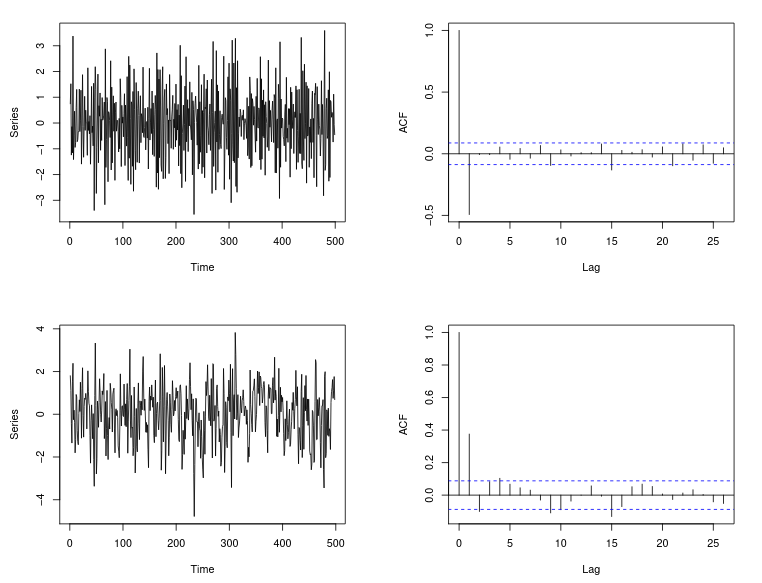
\includegraphics[width=.8\textwidth]{ej-media}
  \caption{Ejemplos de $MA(1)$ (arriba) y $MA(2)$ (abajo) con sus correlogramas respectivos a la derecha.}
  \label{fig:ej-media}
\end{figure}

Observamos como para $MA(1)$ el correlograma muestra valores significativos solo para $\tau = 0, 1$ y para $MA(2)$ para $\tau = 0, 1, 2$, correspondiéndose con nuestro estudio de la función de autocorrelación.

\subsection{Procesos autorregresivos}

Consideramos un modelo que se basa en la idea de las medias móviles de utilizar valores de tiempos pasados, pero en vez de considerarlas de un proceso basado en ruido usaremos el propio proceso (\autoref{def:proceso-autorregresivo}).

\begin{definicion}[Proceso autorregresivo]
  Un proceso $\{X_t\}_{t \in T}$ se dice que es un proceso autorregresivo de orden $p$, notado como $\{X_t\} \sim AR(p)$, si se puede expresar de la siguiente forma:

  $$X_t = \phi_1 X_{t-1} + \ldots + \phi_p X_{t - p} + Z_t = \sum \limits^p_{i = 1} \left(\phi_i X_{t - i}\right) + Z_t, \; \forall t \in T,$$

  donde $\{Z_t\}_{t \in T} \sim WN(0, \sigma^2)$, y coeficientes reales $\{\phi_i\}_{i = 1}^p \subset \R$.
  \label{def:proceso-autorregresivo}
\end{definicion}

Se ha considerado que $\mu = 0$, aunque es posible trabajar con una media no nula. Así, estudiamos el caso más simple $p = 1$, $AR(1)$ expresado como \eqref{eq:ar-simple}

\begin{equation}
  X_t = \phi X_{t - 1} + Z_t, \, \forall t \in T.
  \label{eq:ar-simple}
\end{equation}

Si sustituimos los $X_{t - i}$ mediante recursividad obtenemos \eqref{eq:ar-simple2}

\begin{equation}
  X_t = \phi\left(\phi X_{t-2} + Z_{t-1}\right) + Z_t = \phi^2\left(\phi X_{t-3} + Z_{t-2}\right) + \phi Z_{t-1} + Z_t, \, \forall t \in T.
  \label{eq:ar-simple2}
\end{equation}

Si repetimos este proceso infinitamente entonces \eqref{eq:ar-simple3}

\begin{equation}
  X_t = Z_t + \phi Z_{t-1} + \phi^2 Z_{t-2} + \ldots = \sum \limits^{+\infty}_{i = 0} \phi^i Z_{t - i}, \; \forall t \in T,
  \label{eq:ar-simple3}
\end{equation}

escogido $|\phi| < 1$ para que la suma converja, $AR(1)$ se comporta como un modelo $MA(\infty)$, indicando que hay una cierta dualidad entre los modelos $AR$ y $MA$.

Estudiamos el primer y segundo orden del proceso considerando que las variables $Z_t$ son incorreladas, entonces $\forall t \in T$ se tiene \eqref{eq:ar-momentos}

\begin{gather}
  E[X_t] = 0, \\
  Var[X_t] = \sigma^2 \sum \limits^{+\infty}_{i = 0} \left(\phi^{2i}\right).
  \label{eq:ar-momentos}
\end{gather}

La varianza será finita si $|\phi|^2 < 1$, por lo que al tomar $|\phi| < 1$ se tiene \eqref{eq:ar-var}

\begin{equation}
  Var[X_t] = \dfrac{\sigma^2}{1 - \phi^2}, \; \forall t \in T.
  \label{eq:ar-var}
\end{equation}

La función de autocovarianza viene dada por \eqref{eq:ar-autocovarianza}

\begin{equation}
  \begin{aligned}
    \gamma(\tau) & = E[X_t X_{t + k}] = E\left[\left(\sum \limits^{+\infty}_{i = 0} \phi^i Z_{t - i}\right)\left(\sum \limits^{+\infty}_{i = 0} \phi^i Z_{t + \tau - i}\right)\right] \\
    & = \sigma^2 \sum \limits^{+\infty}_{i = 0} \phi^i \phi^{\tau + i} = \phi^\tau \dfrac{\sigma^2}{1 - \phi^2}.
  \end{aligned}
  \label{eq:ar-autocovarianza}
\end{equation}

Por tanto como $\gamma(\tau)$ no depende de $t$, el proceso $AR(1)$ es un proceso estacionario de segundo orden (bajo la condición de que $|\phi| < 1$). La función de autocorrelación será \eqref{eq:ar-autocorrelacion}

\begin{equation}
  \rho(\tau) = \phi^\tau, \; \tau \in T.
  \label{eq:ar-autocorrelacion}
\end{equation}

Simulemos unos cuantos procesos autorregresivos mediante ruido $Z_t \sim N(0, 1)$: $X_t = \frac{4}{5}X_{t-1} + Z_t$, $X_t = -\frac{4}{5}X_{t-1} + Z_t$ y $X_t = \frac{3}{10}X_{t-1} + Z_t$ cuyas series mostramos de arriba a bajo respectivamente, junto a sus correlogramas en \autoref{fig:ar-simulado} (\cite{chatfield2019analysis}).

\begin{figure}[htpb]
  \centering
  %\hspace*{-2.5cm}
  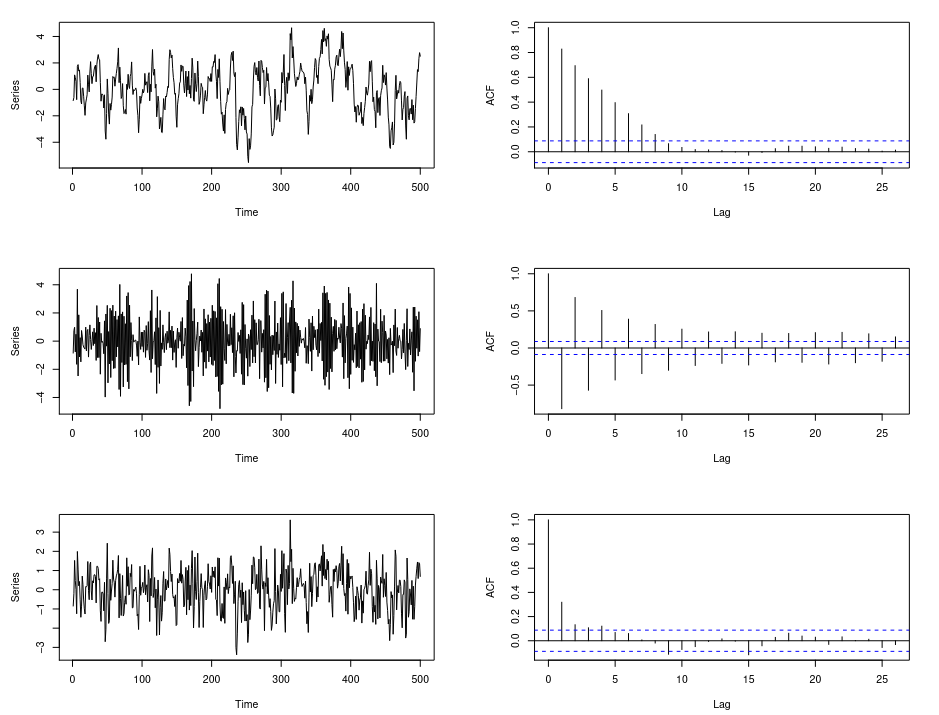
\includegraphics[width=.85\textwidth]{ar-simulado}
  \caption{Ejemplos de $AR(1)$ con varios valores junto con sus correlogramas.}
  \label{fig:ar-simulado}
\end{figure}

Observamos como los correlogramas van convergiendo a 0, decreciendo absolutamente. Cuando $1 > \phi > 0$ (1er y 3er proceso) los valores son todos positivos mientras que cuando $-1 < \phi < 0$ (2o proceso) se van alternando entre positivos (desfase par) y negativos (desfase negativo).

Por otro lado, la función de autocovarianza \eqref{eq:ar-autocovarianza} era posible obtenerla de otra manera. Asumimos de antemano que el proceso es estacionario, entonces $E[X_t]$ debe ser constante (asumamos que es 0). Si multiplicamos el modelo \eqref{eq:ar-simple} por $X_{t-k}$ y tomamos esperanzas obtenemos \eqref{eq:ar-truco}

\begin{equation}
  \gamma(\tau) = \phi \gamma(-\tau + 1), \; \forall \tau > 0,
  \label{eq:ar-truco}
\end{equation}

ya que $E[Z_t X_{t-\tau}] = 0$, $\forall \tau > 0$ debido a la incorrelación de las $Z_t$. Además como $\gamma$ es función par entonces \eqref{eq:ar-truco2}

\begin{equation}
  \gamma(\tau) \phi \gamma(\tau - 1), \; \forall \tau > 0.
  \label{eq:ar-truco2}
\end{equation}

Finalmente como $\gamma(0) = \sigma^2_X$ entonces $\gamma(\tau) = \phi^\tau \sigma^2_X, \; \forall \tau \geq 0$ y además $\rho(\tau) = \phi^\tau, \; \forall \tau > 0$.

Recordando una de las propiedades de $\rho$ cuando el proceso era estacionario se tenía que $|\rho(\tau)| \leq 1, \, \forall \tau \geq 0$ entonces se debe cumplir que $|\phi| \leq 1$. Excluimos el caso degenerado $|\phi| = 1$ y por tanto se debe cumplir que $|\phi| < 1$.

Esta forma alternativa es aplicable para el caso de un modelo $AR(p)$ general, obteniendo Las siguiente ecuaciones para la función de autocorrelación \eqref{eq:ar-general}

\begin{equation}
  \rho(\tau) = \phi_1 \rho(\tau - 1) + \cdots + \phi_p \rho(\tau - p) =
  \begin{cases}
    \sigma^2, & \tau = 0 \\
    0, & 0 < \tau \leq p
  \end{cases}
  \label{eq:ar-general}
\end{equation}

Estas son las llamadas ecuaciones de Yule-Walker \cite{yule1971method, walker1931periodicity}, un conjunto de ecuaciones en diferencias que tienen la solución general \eqref{eq:sol-general}

\begin{equation}
  \rho(\tau) = A_1 \pi_1^{|\tau|} + \cdots + A_p \pi_p^{|\tau|}, \; \forall \tau > 0,
  \label{eq:sol-general}
\end{equation}

donde $\{\pi_i\}_{i = 0}^p$ son las raíces de la ecuación auxiliar \eqref{eq:sol-auxiliar}

\begin{equation}
  y^p - \phi_1 y^{p-1} - \cdots - \phi_p = 0.
  \label{eq:sol-auxiliar}
\end{equation}

Las constantes $\{A_i\}_{i = 0}^p$ se escogen para satisfacer las condiciones iniciales dependientes de $\rho(0) = 1$, que implican que $\sum_{i = 0}^p A_i = 1$. Las $(p - 1)$ primeras ecuaciones de Yule-Walker añaden $(p-1)$ restricciones más en $\{A_i\}_{i = 0}^p$ usando $\rho(0) = 1$ e $\rho(\tau) = \rho(\tau)$.

De la solución \eqref{eq:sol-general} vemos que $\rho(\tau)$ no depende de $t$ por lo que lo único que necesitamos para que el proceso $AR(p)$ sea estacionario es que los $|\pi_i| < 1$, $i = 1, \ldots, p$, que de hecho es una condición necesaria y suficiente.

\subsection{Procesos lineales}

Si generalizamos el funcionamiento de los modelos $AR$ y $MA$ llegamos a los procesos lineales (\autoref{def:proceso-lineal}).

\begin{definicion}[Proceso lineal]
  Un proceso $\{X\}_{t \in T}$ se dice que es un proceso lineal si se puede representar de la siguiente forma:

  $$X_t = \sum \limits^{+\infty}_{i = -\infty} \psi_{j} Z_{t - i}, \; \forall t \in T,$$

  con $\{Z\}_{t \in T} \sim WN(0, \sigma^2)$ y $\{\psi_i\}^{+\infty}_{i = -\infty} \subset \R$ constantes que cumplen que $\sum \limits^{+\infty}_{i = -\infty} |\psi_j| < \infty$.
  \label{def:proceso-lineal}
\end{definicion}

Según los coeficientes $\psi$ se puede obtener cualquier modelo $AR$ o $MA$. Por ejemplo si se toman $\psi = 0, \, \forall i < 0$ entonces el proceso sería $MA(\infty)$.

Veamos entonces que si cualquier proceso lineal es estacionario de segundo orden si lo es el proceso $\{Z_t\}_{t \in T}$, de manera que cualquier proceso $AR$ o $MA$ será estacionario de segundo orden (\autoref{prop:proceso-estacionario}).

\begin{proposicion}
  Sea $\{Y_t\}_{t \in T}$ un proceso estacionario de segundo orden con media 0 y función de autocovarianza $\gamma_Y$. Si $\sum_{i = -\infty}^{+\infty} |\psi_i| < \infty$, entonces el proceso definido por:

  $$X_t = \sum \limits^{+\infty}_{i = -\infty} \psi_i Y_{t - i},$$

  es estacionario de segundo orden con media 0 y función de autocovarianza

  $$\gamma_X(\tau)= \sum \limits^{+\infty}_{i=-\infty}\sum \limits^{+\infty}_{j = -\infty} \psi_i \psi_j \gamma_Y(\tau + j - i), \, \tau \in T.$$

  De hecho si $\{X_t\}_{t \in T}$ es un proceso lineal, se tiene que

  $$\gamma_X(\tau) = \sum \limits^{+\infty}_{i = -\infty} \psi_{i} \psi_{i + \tau}\sigma^2, \, \tau \in T.$$
  \label{prop:proceso-estacionario}
\end{proposicion}

\begin{proof}
  Debido a que la suma absoluta de los coeficientes es finita podemos asegurar que la suma $X_t$ es convergente, $\forall t \in T$ se cumple que

  $$E[|X_t|] \leq \sum \limits^{+\infty}_{i = -\infty} |\psi_j| E[|Y_{t-i}|] \leq \sum \limits^{+\infty}_{i = -\infty} \left(|\psi_j|\right) \sqrt{\gamma_Y(0)} < \infty$$

  Como $E[Y_t] = 0, \, \forall t \in T$ Entonces

  $$E[X_t] = E\left[\sum \limits^{+\infty}_{i = -\infty} \psi_i Y_{t - i}\right] = \sum \limits^{+\infty}_{i = -\infty} \psi_i E[Y_{t-i}] = 0$$

  y además para $\tau \in T$

  $$\begin{aligned}
    E[X_{t+\tau}X_t] & = E\left[\left(\sum \limits^{+\infty}_{i = -\infty} \psi_i Y_{t + \tau - i}\right)\left(\sum \limits^{+\infty}_{i = -\infty} \psi_i Y_{t -i}\right)\right] \\
    & = \sum \limits^{+\infty}_{i = -\infty} \sum \limits^{+\infty}_{j = -\infty} \psi_i \psi_j E[Y_{t+\tau-i}Y_{t-j}] \\
    & = \sum \limits^{+\infty}_{i = -\infty}  \sum \limits^{+\infty}_{j = -\infty} \psi_i \psi_j \gamma_Y(\tau + j - i),
  \end{aligned}$$

  que no depende de $t$ y por tanto $\{X_t\}$ es estacionario de segundo orden. Finalmente si $\{Y_t\}$ es ruido blanco entonces $\gamma_Y(\tau + i - j) = \sigma^2$ si $j = i - \tau$ y 0 en caso contrario, obteniendo el último resultado.
\end{proof}

\subsection{Descomposición de Wold}

Recordemos que estamos con procesos estocásticos, en los que esperamos que haya una cierta componente probabilística. No vamos a definir exactamente cuando un proceso es \textbf{determinista} o \textbf{no determinista} ya que se necesitan conceptos muy complejos. En líneas generales nos vienen a indicar si existe cierta aleatoriedad en el proceso, o bien ya sabemos con seguridad absoluta el resultado que se va a obtener.

En todos los modelos que consideramos siembre buscamos que sean procesos no deterministas y no nos interesan los que sean deterministas. Mediante la descomposición de Wold veremos que cualquier serie estacionaria no determinista se puede expresar de manera única como un proceso que puede convertirse en un proceso lineal (\autoref{th:wold}, \cite{wold1938decomposition})

\begin{teorema}[Descomposición de Wold]
  Sea $\{X_t\}_{t \in T}$ un proceso no determinista estacionario de segundo orden, entonces el proceso se puede descomponer de manera única con los procesos $\{Z_t\}_{t \in T}$, $\{V_t\}_{t \in T}$ y coeficientes $\{\psi_i\}_{i = 0}^{\infty}$ de la siguiente forma

  $$ X_t = \sum \limits^{+\infty}_{i = 0} \psi_i Z_{t - i} + V_t, \, \forall t \in T,$$

  y además se cumple lo siguiente

  \begin{enumerate}
    \item $\psi_0 = 1$ y $\sum^{+\infty}_{i = 0} \psi^2_i < \infty$.
    \item $\{Z_t\}_{t \in T} \sum WN(0, \sigma^2)$.
    \item $Cov(Z_s, V_t) = 0$, $\forall t,s \in T$.
    \item $\{V_t\}$ es un proceso determinista.
  \end{enumerate}
  \label{th:wold}
\end{teorema}

El teorema incluye más condiciones que se cumplen pero se ha simplificado para su mejor entendimiento. Lo que nos expresa el teorema, es que cualquier proceso no determinista se puede representar como un proceso lineal que tiene añadido una parte determinista.

De hecho, esta parte determinista está asociada a la media del proceso por lo que para muchos procesos que ya tienen media 0 entonces nos quedará únicamente un proceso lineal \textbf{puramente determinista}.

\subsection{Procesos ARMA}

Finalmente introducimos uno de los procesos más importantes en el modelado de series temporales: los procesos ARMA (modelos autorregresivos de media móvil). La gran importancia de estos modelos reside en que para una clase grande de funciones de autocovarianza $\gamma$ es posible encontrar un proceso ARMA cuya función de autocovarianza $\gamma_X$ está aproximada.

Este modelo está formado combinando los dos modelos que hemos considerado, $MA$ y $AR$ (\autoref{def:arma}, \cite{whittle1951arma}).

\begin{definicion}[Proceso ARMA]
  Un proceso $\{X_t\}_{t \in T}$ se dice que es un proceso $ARMA(p, q)$ si $\{X_t\}$ es estacionario y se cumple que

  $$X_t = \psi X_{t-1} + \ldots + \psi_p X_{t-p} + Z_t + \theta_1 Z_{t-1} + \ldots + \theta_q Z_{t - q}, \; \forall t \in T,$$

  donde $\{Z_t\}_{t \in T} \sim WN(0, \sigma^2)$ y además los polinomios $\phi(z) = 1 - \phi_1 z - \ldots - \phi_p z^p$ y $\theta(z) = 1 + \theta_1z + \ldots + z_q z^q$ no tienen factores comunes.
\label{def:arma}
\end{definicion}

La condición de que los polinomios no tengan factores comunes se impone para que el modelo no se pueda reducir a uno más simple, así evitamos parámetros redundantes.

Si un modelo $ARMA(p, q)$ cumple que $p = 0$ o que $\phi_i = 0, \, \forall i = 1, \ldots, p$ entonces se convierte en un modelo $MA(q)$. Por el contrario si $q = 0$ o $\theta_i = 0, \, \forall i = 1, \ldots, q$, entonces el modelo sería un $AR(q)$.

En la definición vemos que es esencial que $\{X_t\}$ sea estacionario, haciendo un estudio del proceso se obtiene un teorema que nos asegura la existencia y unicidad con una condición muy simple (\autoref{th:existencia-unicidad-arma}, demostración en \cite{brockwell2002introduction} Sección 3.1).

\begin{teorema}[Existencia y unicidad de ARMA]
  Existe una solución estacionaria $\{X_t\}_{t \in T}$ para el modelo $ARMA(p, q)$, y además es la única, si y solo si

  $$\phi(z) = 1 - \phi_1 z - \cdots - \phi_p z^p \neq 0, \; \forall |z| = 1.$$
  \label{th:existencia-unicidad-arma}
\end{teorema}

Para calcular las funciones de autocovarianza y autocorrelación se vuelve a utilizar el método de las ecuaciones de Yule-Walker, donde la diferencia con los modelos $AR(p)$ reside en que tiene condiciones iniciales diferentes. También es posible utilizar el resultado \autoref{prop:proceso-estacionario}.

Mostramos dos ejemplos simulados de procesos $ARMA$, uno $ARMA(1,1)$ expresado como $X_t = \frac{7}{10}X_{t-1} + Z_t - \frac{2}{5}Z_{t-1}$ con $Z-t \sim N(0, 1)$ y otro $ARMA(2,2)$ con $X_t = \frac{9}{10}X_{t-1} - \frac{1}{2}X_{t-2} + Z_t - \frac{1}{5}Z_{t-1} + \frac{1}{4}Z_{t-2}$ con $Z_t \sim N(0, \frac{1}{2})$ en \autoref{fig:arma-ej} (\cite{chatfield2019analysis}).

\begin{figure}[htpb]
  \centering
  %\hspace*{-2.5cm}
  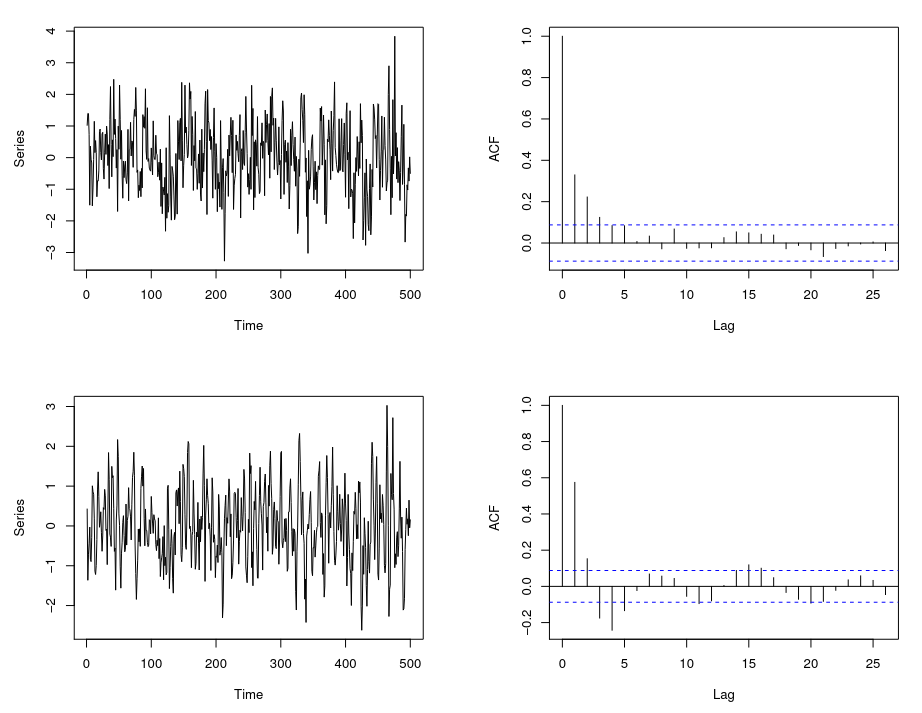
\includegraphics[width=.85\textwidth]{arma-ej}
  \caption{Ejemplos $ARMA(1,1)$ (arriba) y $ARMA(2,2)$ (abajo) con sus correlogramas.}
  \label{fig:arma-ej}
\end{figure}

Hemos obtenido un modelo muy potente con el que podemos adaptar con los parámetros $p$ y $q$ según la serie observada y la función de autocorrelación estimada.

No entraremos en detalles para la realización de predicciones con un modelo $ARMA(p,q)$ debido al largo y complejo desarrollo que debe hacerse, tanto como la estimación de parámetros $\{\phi_i\}$, $\{\theta_i\}$ para adaptar el modelo a la serie observada, como el cálculo de predicciones en base al modelo.

\section{Descomposición}

Una parte importante del análisis de series se centra en el modelado de los procesos mediante la descomposición en varias componentes que suelen exhibir, obteniendo una parte estacionaria al que aplicaremos los modelos vistos. Veremos cuáles son estas componentes y distintas maneras para obtener esta descomposición.

\subsection{Patrones}

Listemos los patrones fundamentales que muestran muchas series:

\begin{itemize}
  \item \textbf{Tendencia}: un cambio a largo plazo en el nivel medio de la serie, que puede ser creciente o decreciente.
  \item \textbf{Variación estacional}: un patrón que se repite cada cierto periodo de tiempo fijo debido a factores estacionales (cada estación, o año).
  \item \textbf{Variaciones cíclicas}: fluctuaciones de las series sin frecuencia fija y que pueden cambiar a lo largo del tiempo.
\end{itemize}

Veamos ejemplos de estos patrones en \autoref{fig:patrones-ej} \cite{hyndman2018forecasting}.

\begin{figure}[htpb]
  \centering
  %\hspace*{-2.5cm}
  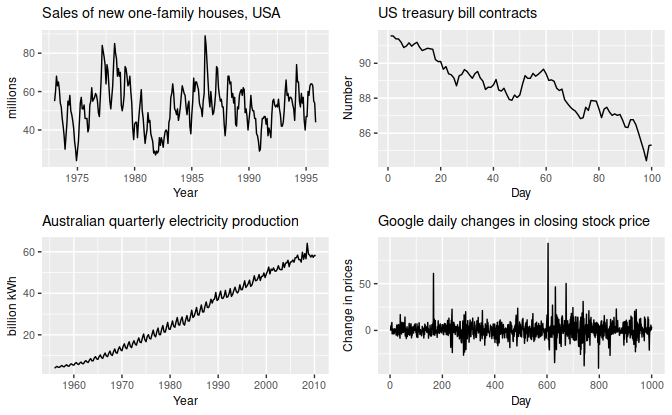
\includegraphics[width=.9\textwidth]{patrones-ejemplos}
  \caption{Ejemplos de series con distintos patrones.}
  \label{fig:patrones-ej}
\end{figure}

Analicemos cada serie para observar los patrones en cada una:

\begin{itemize}
  \item Arriba-izquierda: se muestra un carácter estacional cada año, junto con patrones cíclicos que van variando.
  \item Arriba-derecha: únicamente tendencia decreciente.
  \item Abajo-izquierda: tendencia creciente junto a una variación estacional de un año.
  \item Abajo-derecha: sin ningún patrón observable, son fluctuaciones aleatorias.
\end{itemize}

En base a estos patrones, el análisis clásico de series temporales se basa en la descomposición de estas en los componentes que hemos comentado \eqref{eq:decomposition}

\begin{equation}
  X_t = m_t + s_t + Y_t, \, \forall t \in T,
  \label{eq:decomposition}
\end{equation}

donde $m_t$ es la componente de la tendencia-ciclos (que se dice solamente tendencia), $s_t$ la componente estacional e $Y_t$ ruido aleatorio (débilmente) estacionario.

Esta descomposición se dice que es \textbf{aditiva} pues suma sus componentes y existe otra forma llamada \textbf{multiplicativa}, que suele ser útil cuando las fluctuaciones de la serie son proporcionales al tiempo de la serie \eqref{eq:decomposition-mult}

\begin{equation}
  X_t = m_t \cdot s_t \cdot Y_t, \, \forall t \in T.
  \label{eq:decomposition-mult}
\end{equation}

El enfoque de realizar la descomposición consiste en extraer de las series estas componentes $m_t$, $s_t$ y esperar que el ruido $Y_t$ sea estacionario. Crearemos así un modelo para el proceso estacionario en el que podemos simular valores junto con $m_t$ y $s_t$.

\subsection{Descomposición sin estacionalidad}

Si tenemos un proceso que no presenta la componente estacional entonces obtenemos el siguiente modelo (\autoref{def:solo-tendencia}).

\begin{definicion}[Descomposición con solo tendencia]
  Sea $\{X_t\}$ un proceso entonces una descomposición con solo tendencia está definida por:

  $$ X_t = m_t + Y_t, \; \forall t \in T,$$

  donde $m_t$ es la tendencia e $Y_t$ los residuos y se tiene que $E[Y_t] = 0, \forall t \in T$. Si esto último no fuese así, el modelo se cambiaría por:

  $$ X_t = (m_t + E[Y_t]) + (Y_t - E[Y_t]), \; \forall t \in T.$$
  \label{def:solo-tendencia}
\end{definicion}

\subsubsection{Ajuste polinómico}

Para poder estimar la tendencia $m_t$ podemos utilizar varias técnicas. La primera de ellas es la más simple y conocida: el \textbf{ajuste polinómico} (\autoref{def:ajuste-polinomico}).

\begin{definicion}[Ajuste polinómico]
  Sea un $\{X_t\}_{t = 1}^n$ un proceso y $\{x_t\}_{t = 1}^n$ una serie temporal observada del proceso. El ajuste polinómico de gradp $k$ considera que la tendencia es un polinomio de grado $k$ de la forma

  $$m_t = \sum \limits^k_{i = 0} a_i t^i,$$

  La tendencia estimada $\hat{m}_t$ determinada por los parámetros $\hat{a}_0, \hat{a}_1, \ldots, \hat{a}_k$ se obtienen al minimizar el error cuadrático medio $$\sum \limits^n_{t = 1} (x_t - m_t)^2.$$
  \label{def:ajuste-polinomico}
\end{definicion}

\autoref{fig:ajuste-ej} (\cite{brockwell2002introduction}) nos muestra un ejemplo de ajuste polinómico de grado 2 (cuadrático) donde se estima $\hat{m}_t = \hat{a}_0 + \hat{a}_1 t + \hat{a}_2 t^2$ a través de la serie observada.

\begin{figure}[htpb]
  \centering
  %\hspace*{-2.5cm}
  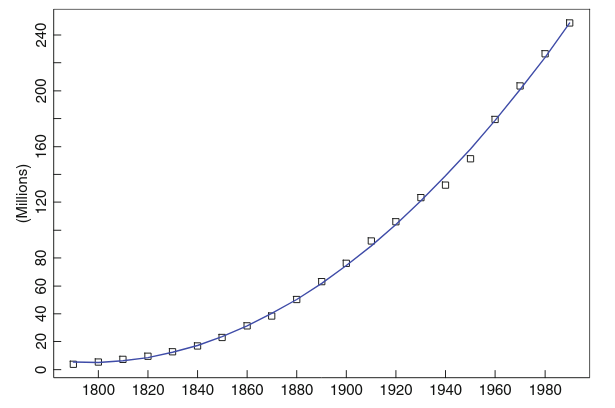
\includegraphics[width=.6\textwidth]{ajuste-ej}
  \caption{Ajuste cuadrático de la población en EE.UU. entre 1790-1990.}
  \label{fig:ajuste-ej}
\end{figure}

\subsubsection{Suavizado con media móvil}

La siguiente técnica consiste en estimar la tendencia mediante el \textbf{suavizado con media móvil} que está basado en el modelo de media móvil (\autoref{def:suavizacion-media}).

\begin{definicion}[Suavizado con media móvil]
  Sea un proceso $\{X_t\}_{t = 1}^n$, y un natural $q \in N$. Se define el proceso suavizado con media móvil simétrica de orden $q$ de $\{X_t\}$ como:

  $$ W_t = \dfrac{1}{2q + 1} \sum \limits^q_{i = -q} X_{t - i}, \, \forall t = 1, \ldots, n.$$
  \label{def:suavizacion-media}
\end{definicion}

Asumiendo que $m_t$ es aproximadamente lineal en el intervalo $[t - q, t + q]$ y que la media de los errores en el mismo intervalo es aproximadamente cero, aplicamos el suavizado al modelo \autoref{def:solo-tendencia} obteniendo \eqref{eq:suavizacion}

\begin{equation}
  W_t = \dfrac{1}{2q + 1} \sum \limits^q_{i = -q} m_{t - i} + \dfrac{1}{2q + 1} \sum \limits^q_{i = -q} Y_{t - i} \approx m_t, \; t = q + 1, \ldots, n - q.
  \label{eq:suavizacion}
\end{equation}

Por tanto la tendencia estimada para un proceso $\{X_t\}_{t = 1}^n$ quedaría como \eqref{eq:suavizacion-estimada}

\begin{equation}
  \hat{m}_t = \dfrac{1}{2q + 1} \sum \limits^q_{i = -q} X_{t - i}, \; t = q + 1, \ldots, n - q.
  \label{eq:suavizacion-estimada}
\end{equation}

Notamos que $\hat{m}_t$ no está definida para $t > n - q$ o $t \leq q$ que podría dejarse así o extender los términos definiendo $X_t := X_1, \forall t < 1$ y $X_t := X_n, \forall t > n$.

Un ejemplo de $\hat{m}_t$ aplicando un suavizado de media móvil con $q = 2$ (5 términos) lo tenemos en \autoref{fig:ej-suavizacion} (\cite{brockwell2002introduction}).

\begin{figure}[htpb]
  \centering
  %\hspace*{-2.5cm}
  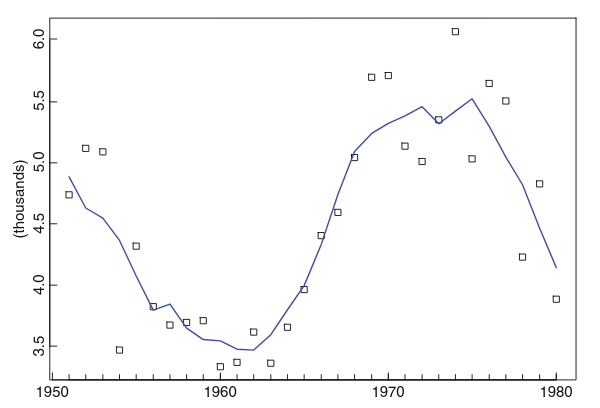
\includegraphics[width=.6\textwidth]{ej-suavizacion}
  \caption{Suavizado con media móvil con 5 términos del número de huelgas en EE.UU entre 1951-1980.}
  \label{fig:ej-suavizacion}
\end{figure}

\subsubsection{Suavizado exponencial}

Finalmente consideramos una técnica que realiza el suavizado como una combinación entre el punto $t$-ésimo actual y el punto estimador anterior (\autoref{def:suavizado-exponencial}).

\begin{definicion}[Suavizado exponencial]
  Sea $\{X_t\}_{t = 1}^n$ un proceso y $\alpha \in [0, 1]$, el suavizado exponencial se define como la estimación de la tendencia del proceso de la siguiente forma:

  $$\hat{m}_t = \alpha X_t + (1 - \alpha)\hat{m}_{t - 1}, \; t = 2, \ldots, n,$$

  donde $\hat{m}_1 = X_1$.
  \label{def:suavizado-exponencial}
\end{definicion}

Este método se denomina suavizado exponencial debido a que $\forall t \geq 2$ se cumple \eqref{eq:exponencial-desarrollada}

\begin{equation}
  \hat{m}_t = \sum \limits^{t - 2}_{i = 1} \alpha(1 - \alpha)^i X_{t - i} + (1 - \alpha)^{t - 1} X_1,
  \label{eq:exponencial-desarrollada}
\end{equation}

donde se puede ver el proceso estimado como una media móvil con pesos decrecientes exponencialmente. Un ejemplo lo tenemos en \autoref{fig:ej-suavizado} (\cite{brockwell2002introduction})

\begin{figure}[htpb]
  \centering
  %\hspace*{-2.5cm}
  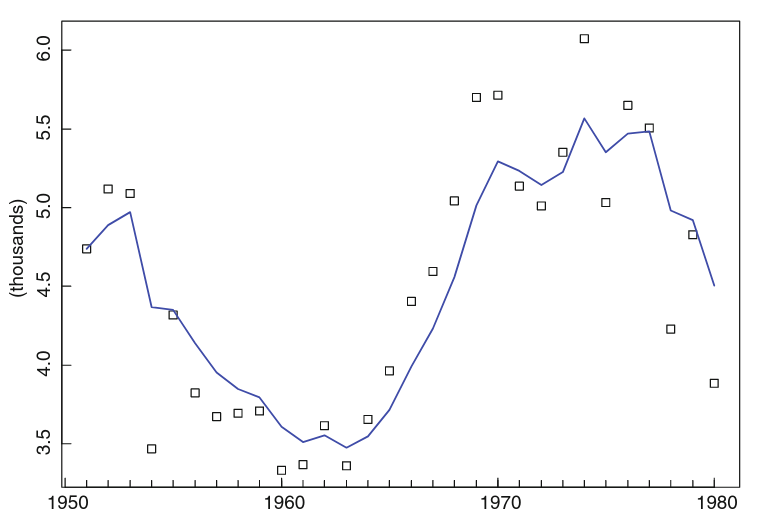
\includegraphics[width=.6\textwidth]{ej-suavizado}
  \caption{Suavizado exponencial con $\alpha = 0.6$ en el número de huelgas.}
  \label{fig:ej-suavizado}
\end{figure}

\subsection{Descomposición completa}

Ahora consideramos la descomposición completa, añadiendo al modelo que hemos estado utilizando la componente estacional. Esperamos que esta componente se repita siempre cada cierto periodo de tiempo $S$ y además que la suma de los valores en un periodo sea cero (\autoref{def:descomposicion-entera}).

\begin{definicion}[Descomposición completa]
  Sea $\{X_t\}$ un proceso entonces una descomposición completa está definida por:

  $$ X_t = m_t + s_t + Y_t, \; \forall t \in T,$$

  donde $m_t$ es la tendencia, $s_t$ es la estacionalidad con periodo $S$ e $Y_t$ los residuos.  Además se tiene que $E[Y_t] = 0$, $s_{t + S} = s_{t}$ y $\sum \limits^{S}_{i = 1} s_i = 0$, $\forall t \in T$.
  \label{def:descomposicion-entera}
\end{definicion}

\subsubsection{Descomposición clásica}

Explicaremos el método clásico básico para obtener una descomposición de un proceso ya que es el funcionamiento básico del resto de descomposiciones que han ido surgiendo.

El primer paso es estimar la tendencia $\hat{m}_t$ mediante una media móvil con pesos especiales para eliminar la estacionalidad y disminuir el ruido. Si el periodo $S$ es par, elegimos $q = S / 2$ y obtenemos la estimación como \eqref{eq:decomp-1}

\begin{equation}
  \hat{m}_t = \dfrac{\dfrac{1}{2}X_{t - q} + X_{t-q+1} + \cdots + X_{t+q+1} + \dfrac{1}{2}X_{t + q}}{S}, \; t = q + 1, \ldots, n - q,
  \label{eq:decomp-1}
\end{equation}

y si el periodo es impar tomamos $q = (d-1)/2$ y estimando como \eqref{eq:decomp-2}

\begin{equation}
  \hat{m}_t = \dfrac{X_{t - q} + X_{t-q+1} + \cdots + X_{t+q+1} + X_{t + q}}{S}, \; t = q + 1, \ldots, n - q.
  \label{eq:decomp-2}
\end{equation}

El siguiente paso es estimar la componente estacional $\hat{s}_t$, para ello primero calculamos la media de las desviaciones de la serie respecto la tendencia estimada \eqref{eq:decomp-3}

\begin{equation}
  w_t = \dfrac{S}{n - 2q} \sum \limits^{\frac{n - q - t}{S}}_{i = \frac{q - t}{S} + 1} \left(X_{t + iS} - \hat{m}_{t + iS}\right), \; t = 1, \ldots, T,
  \label{eq:decomp-3}
\end{equation}

que ajustamos para conseguir que la suma sea 0 \eqref{eq:decomp-4}

\begin{equation}
  \hat{s}_t = w_t - \dfrac{1}{S}\sum \limits^S_{i = 1} w_i, \; t = 1, \ldots, T.
  \label{eq:decomp-4}
\end{equation}

Es posible obtener la serie sin la componente de estacionalidad \eqref{eq:decomp-5}

\begin{equation}
  d_t = X_t - \hat{s}_t, \; t = 1, \ldots, n,
  \label{eq:decomp-5}
\end{equation}

de manera que ahora podemos descomponer $\{d_t\}_{t = 1}^n$ para obtener solamente la tendencia usando un ajuste polinómico. Este paso es posible no realizarlo, pero es interesante tener una forma paramétrica para la tendencia que puede ser extrapolada fácilmente.

Finalmente obtenemos estimamos la componente de residuos \eqref{eq:decomp-6}

\begin{equation}
  \hat{Y}_t = X_t - \hat{m}_t - \hat{s}_t, \; t = 1, \ldots, n.
  \label{eq:decomp-6}
\end{equation}

Un ejemplo de descomposición de un proceso lo tenemos en \autoref{fig:ej-descomposicion} (\cite{hyndman2018forecasting}).

\begin{figure}[htpb]
  \centering
  %\hspace*{-2.5cm}
  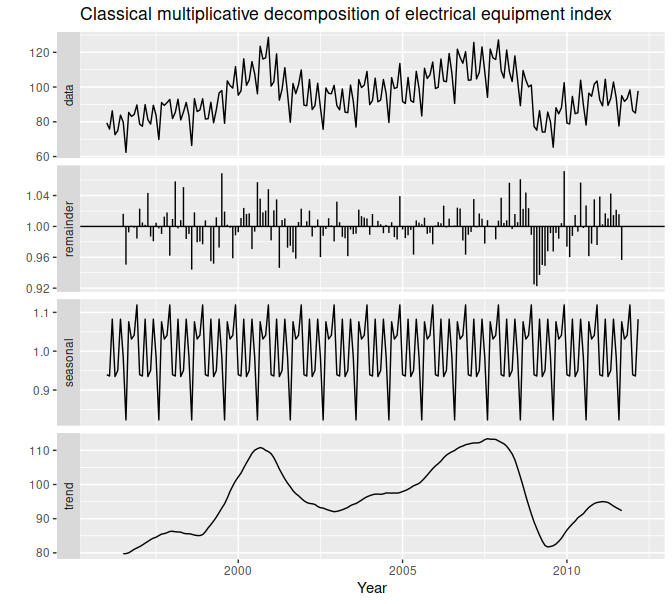
\includegraphics[width=.65\textwidth]{ej-descomposicion}
  \caption{Ejemplo de descomposición clásica de una serie.}
  \label{fig:ej-descomposicion}
\end{figure}

\subsubsection{Otras descomposiciones}

Existen otras descomposiciones que modifican el método que hemos descrito, entre ellas destacan la descomposición X11 \cite{shiskin1965x, dagum2016seasonal} o SEATS (\emph{Seasonal Extraction in ARIMA Time Series}) \cite{gomez1995programs, dagum2016seasonal}.

Una de las descomposiciones más famosas y la que usaremos en el proyecto será la descomposición STL (\emph{Sesonal and Trend decomposition using Loess}) \cite{cleveland1990stl}. Mostramos como ejemplo la descomposición de la serie que habíamos utilizado para la descomposición clásica \autoref{fig:stl-decomposition} (\cite{hyndman2018forecasting}).

\begin{figure}[htpb]
  \centering
  %\hspace*{-2.5cm}
  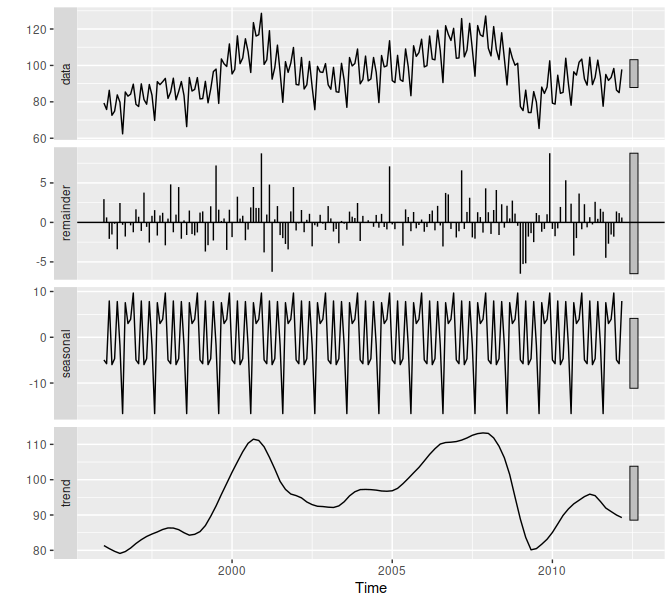
\includegraphics[width=.65\textwidth]{stl-decomposition}
  \caption{Ejemplo de descomposición STL de una serie.}
  \label{fig:stl-decomposition}
\end{figure}

\subsection{Predicción}

Una vez realizada la de composición de un proceso, nos planteamos como poder predecir valores futuros de la serie observada. Mostremos primero alguno de los predictores más simples.

\subsubsection{Predictores simples}

Empecemos primero por el \textbf{método de la media} (\emph{average method}), que considera la media de la serie (\autoref{def:metodo-medio}).

\begin{definicion}[Método de la media]
  Sea un proceso $\{X_t\}_{t = 1}^n$ del cual se toma una serie temporal $\{x_t\}_{t = 1}^n$, se define el método de la media como el predictor dado por

  $$\hat{x}_{n + \tau | n} = \hat{x} = \dfrac{1}{n}\sum \limits^n_{i = 1} x_i, $$

  donde $\hat{x}_{n + \tau | n}$ indica la estimación de $x_{n + \tau}$ en base a los datos $x_1, \ldots, x_n$.
  \label{def:metodo-medio}
\end{definicion}

El \textbf{método del camino aleatorio} (\emph{random walk method}) predice mediante el último valor de la observación (\autoref{def:metodo-ingenuo}).

\begin{definicion}[Método del camino aleatorio]
  Sea un proceso $\{X_t\}_{t = 1}^n$ del cual se toma una serie temporal $\{x_t\}_{t = 1}^n$, se define el método del camino aleatorio como el predictor dado por

  $$\hat{x}_{n + \tau | n} = x_n$$
  \label{def:metodo-ingenuo}
\end{definicion}

Para series con una alta estacionalidad funciona muy bien el \textbf{método de la ingenuidad estacional} (\emph{seasonal naîve method}) en el que se predice tomando la última observación que se corresponde con el periodo de la estacionalidad (\autoref{def:seasonal-naive}).

\begin{definicion}[Método de la ingenuidad estacional]
  Sea un proceso $\{X_t\}_{t = 1}^n$ del cual se toma una serie temporal $\{x_t\}_{t = 1}^n$, se define el método medio como el predictor dado por

  $$\hat{x}_{n + \tau | n} = x_{n + \tau - S(k + 1)},$$

  donde $S$ es el periodo de la componente estacional y $k$ la parte integral de $(\tau - 1)/S$.
  \label{def:seasonal-naive}
\end{definicion}

Finalmente el \textbf{método de deriva} (\emph{drift method}) que modifica el método del camino aleatorio añadiendo una tendencia derivada de la recta extrapolada entre el primer y último dato de la serie (\autoref{def:metodo-deriva}).

\begin{definicion}[Método de deriva]
  Sea un proceso $\{X_t\}_{t = 1}^n$ del cual se toma una serie temporal $\{x_t\}_{t = 1}^n$, se define el método medio como el predictor dado por

  $$\hat{x}_{n + \tau | n} = x_n + \tau \left(\dfrac{x_n - x_1}{n - 1}\right).$$
  \label{def:metodo-deriva}
\end{definicion}

Mostramos un ejemplo de funcionamiento de predicción de los métodos de la media (\emph{mean}, en rojo), del camino aleatorio (\emph{naïve}, en verde) e ingenuo estacional (\emph{seasonal naïve}, en azul) en \autoref{fig:ej-metodos1} (\cite{hyndman2018forecasting}).

\begin{figure}[htpb]
  \centering
  %\hspace*{-2.5cm}
  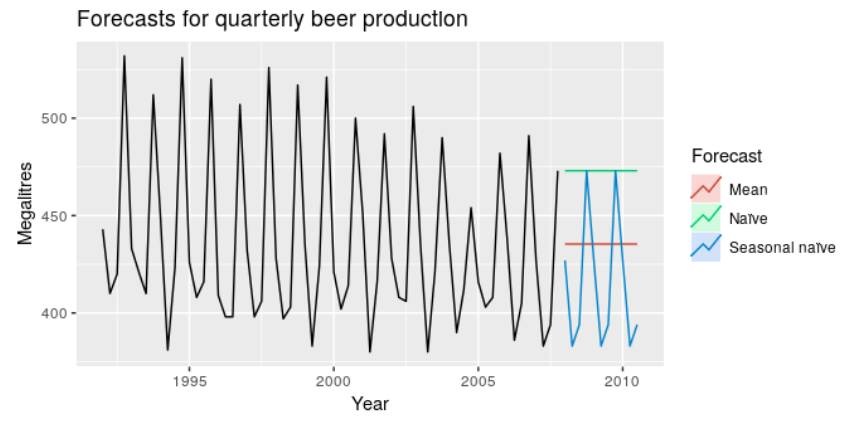
\includegraphics[width=.65\textwidth]{ej-metodos1}
  \caption{Ejemplo de predictores de la media, del camino aleatorio e ingenuo estacional.}
  \label{fig:ej-metodos1}
\end{figure}

Y otro con el método de deriva (\emph{drift}, en rojo), de la media (\emph{mean}, en verde) y del camino aleatorio (\emph{naïve}, en azul) en \autoref{fig:ej-metodos2} (\cite{hyndman2018forecasting}).

\begin{figure}[htpb]
  \centering
  %\hspace*{-2.5cm}
  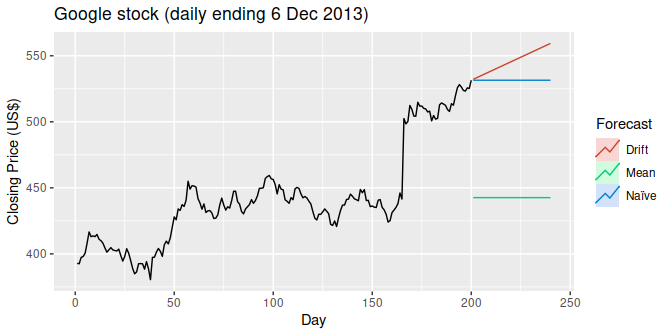
\includegraphics[width=.65\textwidth]{ej-metodos2}
  \caption{Ejemplo de predictores de deriva, de la media y del camino aleatorio.}
  \label{fig:ej-metodos2}
\end{figure}

\subsubsection{Predictores con descomposición}

Cuando nos encontramos con un proceso general $\{X_t\}$ que parece presentar componentes estacionales y tendencia, realizamos una descomposición \eqref{eq:pred-decomp}

\begin{equation}
  X_t = m_t + s_t + Y_t, \; \forall t \in T,
  \label{eq:pred-decomp}
\end{equation}

de manera que hacemos las predicciones por separado para cada componente. Para la estacionalidad $s_t$, debido a su carácter periódico se puede utilizar el predictor ingenuo estacional, para la tendencia $m_t$ podemos predecir con el método de deriva o el método usado para el modelado de la tendencia (ajuste polinómico, suavizado) y finalmente para los residuos $Y_t$ que son estacionarios se puede modelar por ejemplo con un $ARMA$.

También es interesante considerar la descomposición \eqref{eq:decomp-nueva}

\begin{equation}
  X_t = s_t + a_t, \; \forall t \in T,
  \label{eq:decomp-nueva}
\end{equation}

donde $a_t = m_t + Y_t$ es la componente estacionalmente ajustada. En este caso se puede usar el predictor del camino aleatorio y también una modificación de $ARMA$ que veremos más adelante que utiliza otro enfoque para obtener una serie estacionaria.

Veamos un ejemplo de descomposición STL que predice utilizando el método ingenuo estacional para la estacionalidad y el método de camino aleatorio para la componente estacionalmente ajustada, junto con los intervalos de confianza \autoref{fig:stl-predict} (\cite{hyndman2018forecasting}).

\begin{figure}[htpb]
  \centering
  %\hspace*{-2.5cm}
  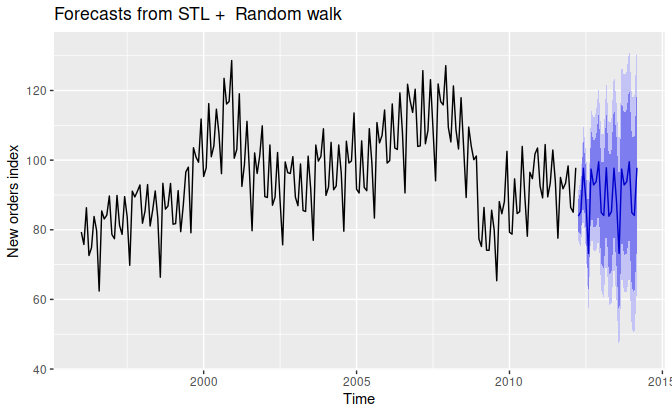
\includegraphics[width=.5\textwidth]{stl-prediccion}
  \caption{Ejemplo de predicción con descomposición STL y método ingenuo estacional y camino aleatorio con intervalos de confianza.}
  \label{fig:stl-predict}
\end{figure}

\section{Diferenciación}

Estudiamos el siguiente método para obtener un proceso estacionario de la serie observada, la \textbf{diferenciación}. Fundamentalmente consiste en aplicar diferencias entre observaciones contiguas de la serie para eliminar la tendencia y/o la estacionalidad, dejando un proceso estacionario.

\subsection{Procesos sin estacionalidad}

Primero veamos como aplicar el método de la diferenciación para procesos que no presentan una componente de estacionalidad, recordando el modelo definido en \autoref{def:solo-tendencia}.

Intentamos eliminar la tendencia usando la diferenciación. Introduzcamos antes  el operador de diferenciación con desfase 1 como \autoref{def:operador-diff}.

\begin{definicion}[Operador diferenciación $\nabla$]

Sea un proceso $\{X_t\}_{t \in T}$, se define el operador de diferenciación con desfase 1, notado como $\nabla$, aplicado al proceso $\{X_t\}$ como la siguiente expresión:

$$\nabla X_t = X_t - X_{t - 1} = (1 - B)X_t, \; \forall t \in T,$$

donde $B$ es el operador de desplazamiento hacia atrás definido por

$$BX_t = X_{t-1}, \; \forall t \in T.$$
\label{def:operador-diff}
\end{definicion}

Las potencias de los operadores se definen como uno podría esperar \eqref{eq:potencias-op}

\begin{gather}
  B^i(X_t) = X_{t-i}, \; \forall i \geq 1, \\
  \nabla^i(X_t) = \nabla(\nabla^{i-1}(X_t)), \; \forall i \geq 1, \\
  \nabla^0(X_t) = X_t.
\label{eq:potencias-op}
\end{gather}

Podemos manipular polinomios de $B$ y $\nabla$ de la misma manera que con polinomios de variables reales, por ejemplo \eqref{eq:diff-ej}

\begin{equation}
  \nabla^2X_t = \nabla(\nabla(X_t)) = (1-B)(1-B)X_t = (1 - 2B + B^2)X_t = X_t - 2X_{t-1} + X_{t-2}.
  \label{eq:diff-ej}
\end{equation}

Sea un proceso $\{X_t\}$ dado por \autoref{def:solo-tendencia} y supongamos que la tendencia es lineal, $m_t = c_0 + c_1t$. Aplicando la diferenciación a $\{X_t\}$ obtenemos \eqref{eq:diff-tendencia}

\begin{equation}
  \nabla X_t = \nabla m_t + \nabla Y_t = c_0 + c_1 t - c_0 - c_1(t - 1) + \nabla Y_t = c_1 + \nabla Y_t, \; \forall t \in T,
  \label{eq:diff-tendencia}
\end{equation}

queda una constante $c_1 \in \R$. Para ver que $\nabla X_t$ sea estacionario podemos ignorarla (la constante es la media), y ver si $\nabla Y_t$ es estacionario \eqref{eq:diff-estacionario}

\begin{equation}
  \begin{aligned}
  Cov[\nabla Y_t, \nabla Y_s] & = Cov[Y_t, Y_s] - Cov[Y_{t-1}, Y_s] - Cov[Y_t, Y_{s-1}] + Cov[Y_{t-1}, Y_{s-1}] \\
  & = \gamma_Y(t - s) - \gamma_Y(t - s - 1) - \gamma_Y(t - s + 1) + \gamma_Y(t - s) \\
  & = 2\gamma_Y(t - s) - \gamma_Y(t - s + 1) - \gamma_Y(t - s - 1), \; \forall t,s \in T,
  \end{aligned}
  \label{eq:diff-estacionario}
\end{equation}

al ser $Y_t$ estacionario. Como la covarianza no depende de $t$ y la media es constante ($c_1$) $\nabla X_t$ es estacionario. Para un ajuste polinómico general, $m_t = \sum \limits^n_{i = 0} c_i t^i$, e $Y_t$ estacionario tenemos que \eqref{eq:diff-general}

\begin{equation}
  \nabla^i X_t = i!c_i + \nabla^i Y_t, \; \forall t \in T,
  \label{eq:diff-general}
\end{equation}

un proceso estacionario con media $i!c_i$. Si la serie se puede ajustar relativamente bien con un polinomio de grado bajo, entonces al aplicar $\nabla$ unas cuantas veces obtendremos una serie estacionaria. En la práctica el orden de diferenciación necesario suele ser de 1 ó 2 nada más.

Un ejemplo lo tenemos aplicando $\nabla^2$ a la serie \autoref{fig:strikes} (\cite{brockwell2002introduction}) que produce la serie \autoref{fig:strikes-diff} \cite{brockwell2002introduction}, sin tendencias aparentes.

\begin{figure}[htpb]
  \centering
  %\hspace*{-2.5cm}
  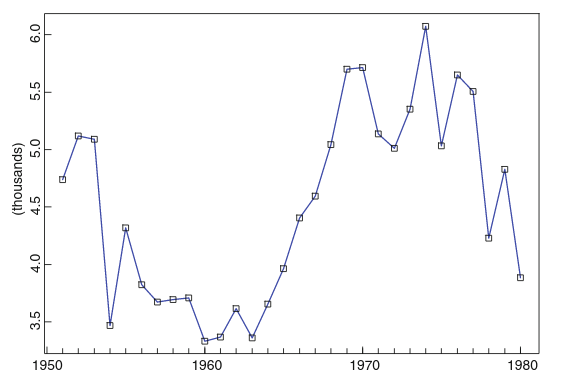
\includegraphics[width=.35\textwidth]{strikes}
  \caption{Huelgas en EE.UU, 1951-1980.}
  \label{fig:strikes}
\end{figure}


\begin{figure}[htpb]
  \centering
  %\hspace*{-2.5cm}
  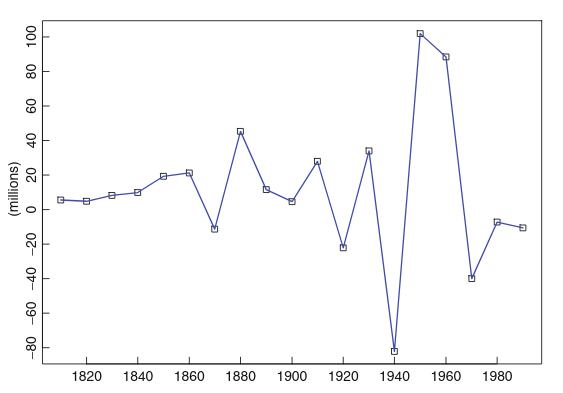
\includegraphics[width=.35\textwidth]{strikes-diff}
  \caption{Segundas diferencias ($\nabla^2$) en la serie de huelgas.}
  \label{fig:strikes-diff}
\end{figure}

\subsection{Procesos con estacionalidad}

Cuando el modelo contiene una componente estacional \autoref{def:descomposicion-entera} con un patrón que se repite cada cierto periodo $S$. Para lidiar con esto podemos extender el operador $\nabla$ que habíamos definido de desfase 1 a un $d$ genérico \autoref{def:diff-estacional}

\begin{definicion}[Operador diferenciación $\nabla_d$]
  Sea un proceso $\{X_t\}_{t \in T}$, el operador de diferenciación con desfase $d$, notado como $\nabla_d$, aplicado al proceso $\{X_t\}$ se define como

  $$\nabla_d X_t = X_t - X_{t - d} = (1 - B^d)X_t, \; \forall t \in T.$$
\label{def:diff-estacional}
\end{definicion}

Considerando un proceso $\{X_t\}$ dado como \autoref{def:descomposicion-entera}, donde el proceso estacional $\{s_t\}$ tiene periodo $S$, entonces podemos aplicar $\nabla_S$ obteniendo \eqref{eq:diff-estacional}

\begin{equation}
  \nabla_S X_t = m_t - m_{t - S} + Y_t - Y_{t - S}, \; \forall t \in T,
\label{eq:diff-estacional}
\end{equation}

mostrando que el proceso $\nabla_S X_t$ no tiene estacionalidad, por lo que se le pueden aplicar los métodos conocidos para los métodos no estacionales. En particular ahora se le puede aplicar una potencia del operador $\nabla$.

Un ejemplo de modelo donde hemos aplicado $\nabla_12 \nabla$ lo tenemos en \autoref{fig:diff-season} (\cite{hyndman2018forecasting}) que se ha aplicado primero una transformación logarítmica, una transformación común para series que aumentan o decrecen con el tiempo (es equivalente a usar un modelo multiplicativo).

\begin{figure}[htpb]
  \centering
  %\hspace*{-2.5cm}
  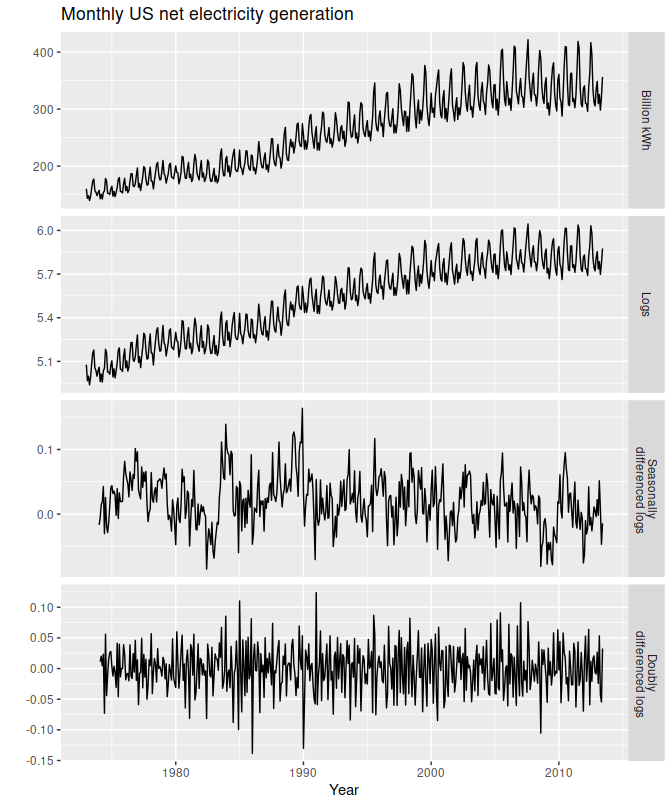
\includegraphics[width=.5\textwidth]{diff-season}
  \caption{Generación de electricidad mensual en EEUU, con transformación logarítmica, diferenciación estacional ($\nabla_{12}$) y una diferenciación ($\nabla$) (de arriba a abajo, respectivamente).}
  \label{fig:diff-season}
\end{figure}

La transformación logarítmica estabiliza las variaciones de la serie, y la diferenciación estacional quita la componente estacional completamente. La diferenciación adicional deja la serie como un proceso estacionario.

\subsection{Modelo ARIMA}

Existe una modificación de los modelos ARMA para considerar directamente el modelado con series sin estacionalidad: el modelo \textbf{ARIMA} (modelos autorregresivos integrados de media móvil) \cite{box2011time}. Juntaremos el modelo ARMA con la idea de realizar una diferenciación $\nabla^d$ para modelar directamente cualquier serie sin estacionalidad \autoref{def:arima}.

\begin{definicion}[Modelo ARIMA]
  Un proceso $\{X_t\}_{t \in T}$ se dice que es un proceso $ARIMA(p, d, q)$ si el proceso definido por

  $$ Y_t = (1 - B)^d X_t, \; \forall t \in T,$$

  es un proceso $ARMA(p, q)$.
\label{def:arima}
\end{definicion}

Mostramos ejemplos $ARIMA$ simulados con sus correlogramas: $ARIMA(1, 1, 1)$ dado por $(1 + \frac{1}{2}B)(1-B)X_t = (1+\frac{3}{10}B)Z_t$ y $ARIMA(1, 1, 2)$ dado por $(1 - \frac{3}{5}B)(1-B)X_t = (1-\frac{3}{10}B+\frac{1}{2}B^2)Z_t$ \autoref{fig:ej-arima} (\cite{chatfield2019analysis}).

\begin{figure}[htpb]
  \centering
  %\hspace*{-2.5cm}
  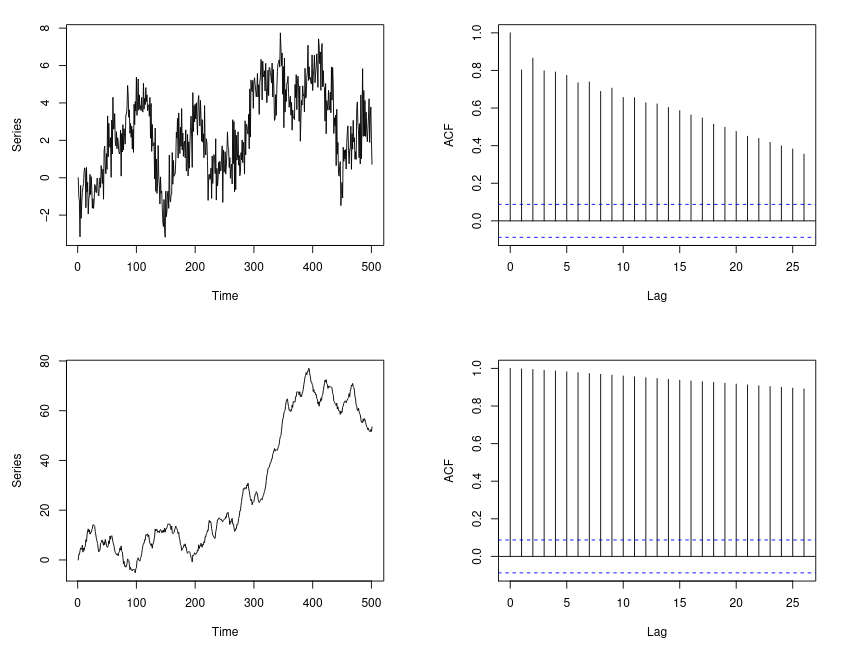
\includegraphics[width=.7\textwidth]{ej-arima}
  \caption{Modelos simulados $ARIMA(1, 1, 1)$ (arriba) y $ARIMA(1, 1, 2)$ (abajo).}
  \label{fig:ej-arima}
\end{figure}

\subsection{Modelo SARIMA}

Si incluimos la diferenciación estacional $\nabla_S$ al modelo ARIMA podremos extender los modelos ARMA para series que manifiestan una componente estacional, este es el modelo \textbf{SARIMA} (Seasonal ARIMA) \autoref{def:sarima} (\cite{box2011time}).

\begin{definicion}[Modelo SARIMA]
  Un proceso $\{X_t\}_{t \in T}$ se dice que es un modelo $SARIMA(p,d,q)\times(P,D,Q)_S$ con periodo $S$ si la serie diferenciada $Y_t = (1 - B)^d(1 - B^S)^D X_t$ es un proceso ARMA definido por

  $$\phi(B)\Phi(B^S)Y_t = \theta(B)\Theta(B^S)Z_t, \; \forall \tau \in T,$$

  donde $\{Z_t\}_{t \in T} \sim WN(0, \sigma^2)$, $\phi(z) = 1 - \phi_1 z - \cdots - \phi_p z^p$, $\Phi(z) = 1 - \Phi_1z - \cdots - \Phi_P z^P$, $\theta(z) = 1 + \theta_1 z + \cdots + \theta_qz^q$ y $\Theta(z) = 1 + \Theta_1z + \cdots + \Theta_Q z^Q$.
\label{def:sarima}
\end{definicion}

Un ejemplo de modelo $SARIMA(3, 0, 1)(0, 1, 2)_12$ predictor en una serie lo tenemos en \autoref{fig:ej-sarima} (\cite{hyndman2018forecasting}) junto a los intervalos de confianza.

\begin{figure}[htpb]
  \centering
  %\hspace*{-2.5cm}
  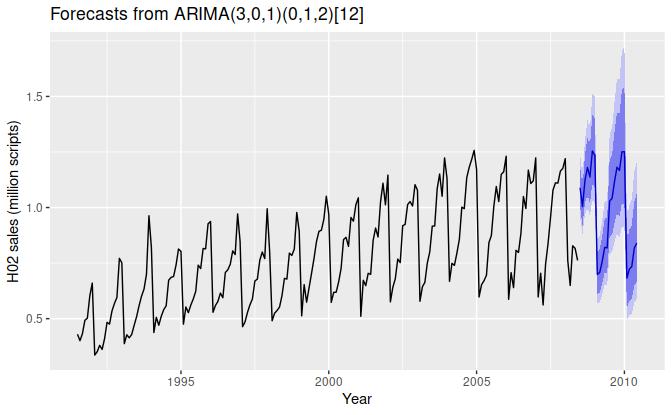
\includegraphics[width=.6\textwidth]{ej-sarima}
  \caption{Predicciones del modelo $SARIMA(3, 0, 1)(0, 1, 2)_12$.}
  \label{fig:ej-sarima}
\end{figure}


\endinput
